\documentclass{article}

% Language setting
% Replace `english^{\prime} with e.g. `spanish^{\prime} to change the document language
\usepackage[UTF8]{ctex}

% Set page size and margins
% Replace `letterpaper^{\prime} with `a4paper^{\prime} for UK/EU standard size
\usepackage[letterpaper,top=2cm,bottom=2cm,left=3cm,right=3cm,marginparwidth=1.75cm]{geometry}

% Useful packages
\usepackage{amsmath}
\usepackage{graphicx}
\usepackage[colorlinks=true, allcolors=blue]{hyperref}

\title{Geophysical Fluid Dynamic}
\author{Wang ZY} % Your name

\begin{document}
\maketitle
\tableofcontents
\newpage

\section{基础动力学}

\subsection{流体动力学}
\subsubsection{描述方法}
1. Lagrange方法和Euler方法

Lagrange方法:微团的物理量$q=q(\vec{x_0};t)$, 表示为初始位置和时间的函数。

Euler方法:场的物理量$q=q(\vec{x},t)$,表示为场点和时间的函数


2. 两种方法的联系

假设某一微团在$t=0$时刻位于空间点$\vec{x_0}$,那么这个微团的轨迹可以表示为
$\vec{r}=\vec{r}(\vec{x_0};t)$,那么对于微团运动到的任意一点$\vec{r}$,
我们有这点的欧拉场速度,即该微团的运动速度。表示为:
$$\vec{u}(\vec{x},t) = \vec{u}(\vec{x_0};t)|_{\vec{r}=\vec{x}}$$

同样我们可以得到加速度在欧拉场下可以写为:

\begin{align}\frac{D\vec{u}}{Dt}&=\frac{1}{\delta t}(\vec{u}(\vec{x}+\delta \vec{x},t+\delta t)-\vec{u}(\vec{x}, t))\\&=\frac{1}{\delta t}(\vec{u}(\vec{x}+\delta \vec{x},t+\delta t)-\vec{u}(\vec{x},t+\delta t)+\vec{u}(\vec{x},t+\delta t)-\vec{u}(\vec{x}, t))\\&=\frac{1}{\delta\vec{x}}\frac{\delta \vec{x}}{\delta t}(\vec{u}(\vec{x}+\delta \vec{x},t+\delta t)-\vec{u}(\vec{x},t+\delta t))+\frac{1}{\delta t}(\vec{u}(\vec{x},t+\delta t)-\vec{u}(\vec{x},t+\delta t))\\&=(\vec{u}\cdot\nabla)\vec{u}+\frac{\partial \vec{u}}{\partial t}\end{align}


3. 迹线、流线、脉线

轨迹trajectory:微团的运动轨迹

流线streamline:流速场的连线

脉线streakline:某段时间内经过同一个固定场点的连线

\subsubsection{散度,涡度,剪切应变率}

对于流体微团,我们有速度梯度张量写成对称矩阵S和反对称矩阵A:
$$\nabla\vec{u} = \begin{bmatrix}
\nabla u\\
\nabla v\\
\nabla w
\end{bmatrix}  = \begin{bmatrix}
\frac{\partial u}{\partial x}\ \frac{\partial u}{\partial y}\ \frac{\partial u}{\partial z} \\
\frac{\partial v}{\partial x}\ \frac{\partial v}{\partial y}\ \frac{\partial v}{\partial z} \\
\frac{\partial w}{\partial x}\ \frac{\partial w}{\partial y}\ \frac{\partial w}{\partial z}
\end{bmatrix}  = \begin{bmatrix}
\frac{\partial u}{\partial x}&
\frac{1}{2}(\frac{\partial u}{\partial y}+\frac{\partial v}{\partial x})&
\frac{1}{2}(\frac{\partial u}{\partial z}+\frac{\partial w}{\partial x})\\
\frac{1}{2}(\frac{\partial v}{\partial x}+\frac{\partial u}{\partial y})&
\frac{\partial v}{\partial y}&
\frac{1}{2}(\frac{\partial v}{\partial z}+\frac{\partial w}{\partial y}) \\
\frac{1}{2}(\frac{\partial w}{\partial x}+\frac{\partial u}{\partial z})&
\frac{1}{2}(\frac{\partial w}{\partial y}+\frac{\partial v}{\partial z})&
\frac{\partial w}{\partial z}
\end{bmatrix}+\begin{bmatrix}
0\ 
\frac{1}{2}(\frac{\partial u}{\partial y}-\frac{\partial v}{\partial x})\ 
\frac{1}{2}(\frac{\partial u}{\partial z}-\frac{\partial w}{\partial x})\\
\frac{1}{2}(\frac{\partial v}{\partial x}-\frac{\partial u}{\partial y})\
0\
\frac{1}{2}(\frac{\partial v}{\partial z}-\frac{\partial w}{\partial y}) \\
\frac{1}{2}(\frac{\partial w}{\partial x}-\frac{\partial u}{\partial z})\
\frac{1}{2}(\frac{\partial w}{\partial y}-\frac{\partial v}{\partial z})\
0
\end{bmatrix} $$

这里$tr(S) = \text{div}\vec{u}, L(A) = \frac{1}{2}\text{curl}\vec{u}, L(S)=\frac{1}{2}\text{shear}\vec{u}$,分别对应散度,旋度和剪切应变率

1. 散度(divergence)

散度表示空间个点矢量场发散的强弱程度,大于$0$表示向外发散,小于$0$表示向内吸收,等于$0$表示无源。
散度定义为:$$\text{div} \vec{F} = \nabla\cdot\vec{F}$$

对于一个流体微团来说,速度的散度表示它的体积变化率:
$$\frac{dV}{dt} = \iint_S \vec{u}\cdot d\vec{S} = \iiint_V \nabla\cdot\vec{u} dV$$

2. 涡度/旋度(curl)

涡度描述流体的旋转情况,大小为角速度的两倍,为矢量场。在大气和海洋中,由于垂向和水平方向的量级不同,通常取垂向分量表示涡度,大于$0$表示逆时针旋转,小于$0$表示顺时针旋转。涡度定义为:
$$\text{curl} \vec{F} = \nabla \times \vec{F}$$

对于一个流场来说,围绕其一圈的环量等于其旋度:
$$C = \oint_l \vec{u}\cdot d\vec{l} = \iint_S (\nabla\times\vec{u})\cdot d\vec{S}$$

3. 剪切变形率(shear deformation)

当杆件在两相邻的横截面处有一对垂直于杆轴,但方向相反的横向力作用时,其发生的变形
为该两截面沿横向力方向发生相对的错动,此变形称为剪切变形。

\subsubsection{控制方程}

1. 动量方程

基于牛顿第二定律,$F=ma$,不难得到流体微团质点的加速度:
$$\frac{d\vec{u}}{dt} = -\frac{1}{\rho}\nabla p + \nabla\Phi+\vec{F}$$

其中,$-\frac{1}{\rho}\nabla p$为压强梯度力,$\nabla\Phi$为位势,$\vec{F}$ 为流体微团受到的合外力。

2. 连续方程

基于质量守恒,对于一个流体微团的总质量:
$$\frac{d\delta m}{dt} = \delta V\frac{d\rho}{dt} +\rho\frac{d\delta V}{dt}=0$$

基于1.1.2中的体积变化率方程,$\delta V \rightarrow 0$我们得到:
$$\frac{d\delta V}{dt} = \nabla\cdot\vec{u} \delta V$$

从而:
$$\frac{d\rho}{dt} +\rho\nabla\cdot\vec{u}=0$$

3. 内能方程

基于热力学第一定律:$\delta Q = dI + pd\alpha$,其中$Q$为流体微团获得的总热量,$I$表示流体微团内能的增量,$p\text{d}\alpha$为流体微团向外膨胀做的体积功,$\alpha = 1/\rho$。

对于流体微团,那么有:$$\frac{dI}{dt} = \Omega - p\frac{d\alpha}{dt} 
= \Omega + \frac{p}{\rho^2}\frac{d\rho}{dt}
=\Omega - \frac{p}{\rho}\nabla\cdot\vec{u}$$

其中,$\Omega$为流体微团的加热率。

4. 熵

熵流分为物质流入流出的质熵流和热量流入流出的热熵流,以及由于耗散效应引起的熵产,即:
$$d\eta = d\eta_f + d\eta_g = (\delta_q + \delta_m) + d\eta_g $$

可以得到输入的热量,包含非绝热加热和由于成分变化带来的:
$$dQ = Td\eta + \mu dS$$

从而得到熵方程:
$$T\frac{d\eta}{dt}=\Omega-\mu\frac{dS}{dt}$$

5. 示踪方程

示踪物以及其非保守的源和汇的关系,它们的浓度变化为:
$$\frac{dS_k}{dt} = S^{(k)}$$

6. 状态方程

流体微团的密度和温度、压强以及其示踪物的关系,表示为:
$$\rho = \rho(T,p,S)$$

对于大气可以采用理想近似:$pV=RT$。

对于海洋一般采用经验公式:$\rho = \rho(p,T,S)$,其中$S$为盐度。

\subsubsection{初始条件和边界条件}
初始条件即流体微团的初始状态,边界条件即流体在边界上需要满足的条件。

运动边界条件:边界由连续分布的质点组成,可以变形,但始终都是由这些质点组成;所以, 流体要么平行于边界运动,要么垂直于边界且流体速度必须与边界速度相同。

常用的边界条件:

1. 固壁边界(边界静止不变)$\Rightarrow$底边界,侧边界
$$\vec{u}\cdot\hat{n} = 0$$

2. 滑动边界
$$\vec{u}\cdot\hat{n}=\frac{d\vec{x_0}}{dt}\cdot\hat{n}$$

3. 自由面边界$\Rightarrow$海表,大气底层
基准面高偏离度:
$$z=h(x,y,t)$$
$$=>w=\frac{dz}{dt}=\frac{dh}{dt}$$

\subsubsection{能量守恒}

1. 动能

动能密度:
$$KE=\frac{1}{2}\rho\vec{u}^2$$

联合动量方程和连续方程不难得到:
$$\frac{\partial}{\partial t}\frac{1}{2}\rho\vec{u}^2
+\nabla\cdot\left(\vec{u}(p+\frac{1}{2}\rho\vec{u}^2)\right)
=p\nabla\cdot\vec{u}-g\rho w+\rho\vec{u}\cdot\vec{F}$$

2. 势能

势能密度:
$$PE = \rho gz$$

根据密度方程不难得到:
$$\frac{\partial}{\partial t} \rho gz
+ \nabla\cdot\left(\vec{u}(\rho gz)\right)
=\rho gw $$

3. 内能

内能密度:
$$IE = \rho I$$

联合密度方程和内能方程有:
$$\frac{\partial}{\partial t} \rho I
+ \nabla\cdot(\vec{u}(\rho I))
=\rho\Omega - p\nabla\cdot\vec{u}$$

从而得到总能量密度:
$$E = PE+KE+IE=\frac{1}{2}\rho\vec{u}^2+\rho gz+\rho I$$

根据动能,势能和内能密度方程有:
$$\frac{\partial}{\partial t} (\frac{1}{2}\rho\vec{u}^2+\rho gz+\rho I)
+\nabla\cdot\left(\vec{u}(\frac{1}{2}\rho\vec{u}^2+\rho gz+\rho I+p)\right)
=\rho \Omega + \rho\vec{u}\cdot\vec{F}$$




\subsection{海洋近似}
不可压近似、Boussinesq近似、准静力近似、地转近似。

\subsubsection{质量和密度}
1. 海水不可压缩性:

根据连续性方程,有:
$$\frac{1}{\rho}\frac{d\rho}{dt}+\nabla\cdot\vec{u}=0$$

在海洋中,对于$$\frac{1}{\rho}\frac{d\rho}{dt}\sim\frac{\delta \rho}{\rho}\frac{V}{L} \ll \frac{V}{L}$$

即密度变化对散度的影响很小,从而得到近似的海水不可压缩方程(体积守恒)。
$$\nabla\cdot\vec{u}=0$$

在海洋中,体积守恒的精确度很高,且不需要发展密度项,因此常用于大部分的海洋模式。

2. 速度势函数

基于不可压缩方程,我们可以将速度Helmholtz分解为:

$$\begin{cases}
u = -\frac{\partial\psi}{\partial y}-\frac{\partial^2 \chi}{\partial x\partial z}\\
v = \frac{\partial\psi}{\partial x}-\frac{\partial^2 \chi}{\partial y\partial z}\\
w = \frac{\partial^2 \chi}{\partial x^2} + \frac{\partial^2 \chi}{\partial y^2}
\end{cases}$$

其中,$\psi$为流函数,$\Delta \psi = \hat{k}\cdot\nabla\times\vec{u}$。$\chi$为辐散速度势 divergent velocity potential。

3. 线性化的状态方程

对于海水中的状态方程,常用经验公式来表达,简单情况下可以基于参考态线性展开,有:
$$\rho = \rho_0\left(1 - \alpha(T-T_0) + \beta(S-S_0) + \gamma(p-p_0)\right)$$

一般取$\rho_0=10^3 kg/m^3$,$T_0=10^{\circ}C$,$S_0 = 35ppt$。热膨胀系数$\alpha=2\times10^{-4}K^{-1}$,盐度收缩系数$\beta = 8\times10^{-4}ppt^{-1}$,海水压缩系数$\gamma = 4.5\times10^{-10} Pa^{-1}$。

对于一个流体微团,它的温度变化$5\text{K}$,盐度变化$1\text{ppt}$,深度变化$1000\text{m}$造成的密度变化均在$\delta\rho/\rho\sim 10^{-3}$,由于海水微团很少产生这么大的深度变化,因此,位势密度可以写作:

Boussinesq状态方程:
$$\rho = \rho_0(1-\alpha(T-T_0) + \beta(S-S_0))$$


\subsubsection{海水运动方程简化}
对动量方程采用Boussinesq近似(除了在地心引力项和状态方程中,其它位置的$\rho$都可以由$\rho_0$替代)简化动量方程。同时,对于内能方程,考虑在海洋中,温度对内能的影响,在固定的位置往往是定压的(海水的压强随深度变化很大),从而内能可以写作$I=c_pT$的形式,从而:
$$\begin{cases}
    \frac{d\vec{u}}{dt} = -\frac{1}{\rho_0}\nabla\phi-\frac{\rho}{\rho_0}g\hat{k}+\vec{F}\\
    \nabla\cdot\vec{u} = 0\\
    \frac{dS}{dt} = S^{(k)}\\
    c_p\frac{dT}{dt} = \Omega\\
    T\frac{d\eta}{dt} = \Omega -\mu\frac{dS}{dt}\\
    \rho = \rho_0(1-\alpha(T-T_0) + \beta(S-S_0))
\end{cases}$$
优点

- 滤除了直接与可压缩性有关的现象(如声波、大气中的深对流)

(对于马赫数$M=V/C$)其中$V$为流速,$C$为声速,海洋中马赫数远小于$1$,因此可以忽略声波的影响。

- 状态方程对扰动变量来说是线性化的

(有时会需要更准确的状态方程,对于实际情况,常常会有cabelling instability(不同温度盐度但是相同密度的海水混合,密度降低))

- 变系数方程转化为常系数方程,降低了非线性

- 能量方程的形式比较简单

绝热条件:在$\Omega$和$S^{k}$为$0$时,流体的运动被称为绝热运动,否则为非绝热运动。

在绝热运动下,$T,\eta,S,\rho$均守恒。因此,绝热运动也称为等熵运动。

\subsubsection{边界条件}

1. 运动边界条件

海表边界条件(自由面边界条件):$$w=\frac{dh}{dt}$$

海底边界条件(固壁边界条件):$$\vec{u}\cdot\hat{n}=0$$

刚盖近似边界条件:$w(x,y,0,t)=0$

该近似没有考虑来自近似模式的海表重力波,对于在更大空间和更短的时间尺度上运动的流体来说是十分准确的。
该近似的根据:1)海表高度的变化相对较小;2)海表重力波与更大尺度、更慢的潮流之间的动力相互作用薄弱。

2. 连续边界条件

即大气底部和海表压强连续$p|_{z=h}=p_{atm,0}\approx10^{5}Pa$

反变气压计响应(inverse barometer response):

海表高度变化抵消大气压强的变化,则沿着一个水平面,
在水里空气和水的压强组合在空间和时间上均匀分布,
这样海洋不会出现由于水平气压梯度力作用导致的海洋加速度。

3. 通量边界条件

示踪通量边界条件:
$$\tau(z=-H(x,y))=0$$
$$\tau(z=h(x,y))\ne0$$

动量通量边界条件:

自由滑动边界条件,动量通量为$0$;无滑移边界条件,动量通量不为$0$。

\subsection{大气近似}
\subsubsection{理想气体}
1. 理想气体近似

理想气体的状态方程可以写为:
$$\rho = \frac{p}{RT}$$

其中$R$为干空气比气体常数$R=287 \  m^2s^{-2}K^{-1}$

内能方程,能量输入分为体积功和内能增长,因此,此处的内能增量有定容比热容得到$I=c_vT$。
$$\frac{dI}{dt}=c_v\frac{dT}{dt}=\Omega-RT\nabla\cdot\vec{u}$$

熵方程,考虑与外界没有物质交换:
$$T\frac{d\eta}{dt}=\Omega=c_v\frac{dT}{dt}+RT\nabla\cdot\vec{u}=c_v\frac{dT}{dt}+p\frac{d}{dt}\left(\frac{RT}{p}\right)=c_p\frac{dT}{dt}-\frac{1}{\rho}\frac{dp}{dt}$$

其中$c_p = c_v+R=1004 \ m^2s^{-2}K^{-1}$

对于绝热运动,有:
$$\frac{c_p}{T}\frac{dT}{dt}-\frac{R}{p}\frac{dp}{dt}=0$$

从而得到位温的表达式:

位温和位势密度:
$$\theta=T\left(\frac{p_0}{p}\right)^{R/c_p}$$
$$\rho_{pot} =\frac{p_0}{R\theta}=\rho\left(\frac{p_0}{p}\right)^{c_v/c_p}$$

2. 声波

假设声波的微小扰动,导致的气体运动皆为绝热运动。对于位势密度:
$$\frac{d\rho_{pot}}{dt}=-\frac{\rho_{pot}}{\theta}\frac{d\theta}{dt}=-\frac{\rho_{pot}\Omega}{c_pT}=0$$
即:
$$\frac{d\rho_{pot}}{dt}=\frac{d}{dt}\rho\left(\frac{p_0}{p}\right)^{c_v/c_p}=0$$
$$\frac{d\rho}{dt}-\frac{c_p\rho}{c_vp}\frac{dp}{dt}=0$$
其中$C_s=\sqrt{\frac{c_vp}{c_p\rho}}$为绝热声速或Laplace声速。

考虑对动量方程和密度方程,取一阶的扰动项,有:
$$\frac{\partial \vec{u^{\prime}}}{\partial t}=-\frac{1}{\rho_0}\nabla p^{\prime}$$
$$\frac{\partial\rho^{\prime}}{\partial t}+\rho_0\nabla\cdot\vec{u^{\prime}}=0$$

以及对上式:
$$\frac{\partial\rho^{\prime}}{\partial t}-C_s^{-2}\frac{\partial p^{\prime}}{\partial t}=0$$

不难得到:
$$\frac{\partial^2 p^{\prime}}{\partial t^2}-C_s^2\Delta p^{\prime}=0$$

1)描述具有任意波形的小振幅扰动的传播,波速为$C_s$,且具有任意的传播方向;

2)传播过程中波形不变,故声波为非频散波;

3)对于海洋,当不采用不可压缩近似时,可以得到类似的声波传播形式,海洋中声波的传播速度$C_s$大约为$1500 \ ms^{-1}$


\subsubsection{分层大气}

对于各向速度为$0$的静止大气,动量方程仅在垂向上非平凡,有:
$$\frac{\partial p}{\partial z}+\rho g = 0$$

即静力平衡的微分形式,它表明某一点的压强近似等于该点以上单位截面空气柱的重量(假设外太空空气无重量)。

1. 等熵大气

我们考虑大气和大气之间只有绝热运动,即不同层之间等熵,那么基于1.3.1中的理想气体近似,我们有:
$$\frac{c_p}{T}\frac{dT}{dt}-\frac{R}{p}\frac{dp}{dt}=0$$
$$\frac{c_p}{T}\frac{dT}{dz}-\frac{R}{p}\frac{dp}{dz}=0$$
$$\frac{dT}{dz}=-\frac{g}{c_p}\approx10^{-2}Km^{-1}$$

即温度随着高度升高而降低。在$z=0$时,$T=\theta_0$,有温度的表达式:
$$T=\theta_0-\frac{gz}{c_p}$$
考虑位势密度:
$$\rho_{pot} =\frac{p_0}{R\theta}=\rho(\frac{p_0}{p})^{c_v/c_p}=\rho_{pot,0}(1-\frac{gz}{c_p\theta_0})^{R/c_v}$$

在$z=c_p\theta_0/g\approx3\times10^4m$时,位势密度为$0$,得到等熵大气的高度。

2. 等温大气

简单假设大气等温,那么可以得到大气密度:
$$\rho = \frac{p}{RT}=\frac{p}{RT_0}$$
$$\frac{d\rho}{dz}=\frac{dp}{RT_0dz}=-\frac{\rho g}{RT_0}$$

得到大气密度:
$$\rho = \rho_0 e^{-z/H_0}$$

大气标高$H_0=RT_0/g\approx10^4m$,等温大气可以延伸到无穷远的高度。且有位温:
$$\theta = T_0e^{Rz/c_pH_0}$$

真实大气的分布更接近于等温大气,稳定分层,且位温随高度升高。

\subsubsection{浮力震荡和对流}

浮力振荡:在稳定层结大气中,气块受扰后发生垂直位移离开平衡位置时,将在一个指向平衡位置的净浮力作用下做绝热浮力振荡。

假设环境的气压和密度分别为$\rho_r(z), p_r(z)$,一个气块偏离其平衡位置$z_0, \delta z$的位移,那么这个运动在垂直方向上满足:
$$\frac{dw}{dt}=\frac{d^2\delta z}{dt^2}=-g-\frac{1}{\rho}\frac{\partial p}{\partial z}$$

假设气块的气压始终和环境气压平衡,那么这个气块受到的浮力
$$\frac{d^2\delta z}{dt^2}=g\frac{\rho_r(z_0+\delta z)-\rho_r(z_0)}{\rho_r(z_0)}
=g\frac{1}{\rho_r}\frac{d\rho_r}{dz}\delta z$$

由于密度随高度增高而降低,我们得到浮力频率:
$$N^2=-g\frac{d}{dz}ln(\rho_r)$$

1)$N^2$称为浮力频率或布伦特-维赛拉(Brunt-Vaisala)频率;

2)当$N^2>0$时,表明随高度减小,即密度大的空气位于密度小的空气下方,层结稳定,此时气块将围绕平衡位置做垂直浮力振荡,振荡周期为$P=2\pi/N$;浮力振荡是重力波的一种简单形式:

3)当$N^2<0$时,表明随高度增加,层结不稳定,此时气块将远离平衡位置,形成对流或垂直不稳定。

4)N与真实温度垂直递减率和绝热递减率的差有关

5)热带外对流层中,$N\sim10^{-2}s^{-1}$,相应的振荡周期P约为10min;平流层中N更大

6)对于密度跃层之上的上层海洋,$N\sim10^{-2}s^{-1}$;但在海表附近的混合层一般T和S分布均匀,$N\sim0$;在深海$N^2$一般为正值,但是大小比密度跃层之上的$N^2$小


\subsubsection{静力平衡}

静力平衡关系对于静止大气来说是精确成立的;对于水平尺度远远大于垂直尺度的大尺度流体运动来说,该平衡关系也是近似成立的,即压强梯度力和重力的二力平衡:
$$\frac{\partial p}{\partial z}=-g\rho\begin{cases}
1. resting\\
2. H/L \ll 1
\end{cases}$$

当$H/L \ll 1$,动量方程的垂向加速度可以忽略。

\subsubsection{压强坐标系}
静力近似是建立压强坐标系的数学条件和物理基础,对于中、大尺度的运动来说,这种近似是较为精确的。在气压$p$坐标系下,坐标变量为$(x,y,F(p),t)$,其中,$F(p)$往往为一个单调函数,常用的形式有:
$$\begin{cases}
F(p) = \frac{p_0-p}{g\rho_0}\\
F(p) = H_0(1-(\frac{p}{p_0})^{R/c_p}) (isentropic)
\end{cases}$$


\subsection{地球的旋转特性}

\subsubsection{旋转坐标系}
小尺度运动一般受旋转影响不大,因为小尺度运动的时间尺度比旋转周期小得多;

大尺度运动受旋转的影响比较显著。由于大尺度运动水平特征尺度比垂直特征尺度大很多,因而一般仅仅地球的旋转向量的垂直分量在动力学上是重要的。

我们假设地球的中心存在一个绝对静止的惯性坐标系,那么在地球表面上任意一点,都会围绕地轴惯性坐标系做$\vec{\Omega}$的旋转。

我们取地球表面的旋转坐标系$O_ex_ey_ez_e$和绝对惯性坐标系$O_ax_ay_az_a$,我们有:

任意位矢:
$$\vec{r_a} = \vec{R} + \vec{r_e}$$

其中$\vec{R}$对于旋转坐标系来说为常矢量,对于惯性坐标系来说为变矢,表示旋转坐标系到绝对惯性坐标系的位矢,且有:
$$\vec{r_a} = x_a\hat{i_a} + y_a\hat{j_a} + z_a\hat{k_a}$$
$$\vec{r_b} = x_e\hat{i_e} + y_e\hat{j_e} + z_e\hat{k_e}$$

对于三个方向的旋转坐标基矢量,它们在绝对坐标系下的速度:
$$\frac{d_a}{dt}\hat{i_e} = \vec{\Omega}\times\hat{i_e} $$
$$\frac{d_a}{dt}\hat{j_e} = \vec{\Omega}\times\hat{j_e} $$
$$\frac{d_a}{dt}\hat{k_e} = \vec{\Omega}\times\hat{k_e} $$

从而我们可以得到,相对位矢在绝对坐标系下的速度:
$$\frac{d_a}{dt}\vec{r_e} = \frac{d_ax_e}{dt}\hat{i_e} +\frac{d_ay_e}{dt}\hat{j_e} +\frac{d_az_e}{dt}\hat{j_e}+ x_e \vec{\Omega}\times\hat{i_e}+ y_e \vec{\Omega}\times\hat{j_e}+ z_e \vec{\Omega}\times\hat{k_e}=\frac{d_e}{dt}\vec{r_e}+\vec{\Omega}\times\vec{r_e} $$

不难看出,上述的操作对任意向量成立,即:
$$\frac{d_a}{dt} \vec{A} = \frac{d_e}{dt} \vec{A} + \vec{\Omega}\times\vec{A}$$

令$\vec{A}=\frac{d_a}{dt}\vec{r_a}$,可以得到:
\begin{align}
\frac{d_a}{dt} \frac{d_a}{dt}\vec{r_a} &=\frac{d_e}{dt} \frac{d_a}{dt}\vec{r_a} + \vec{\Omega}\times\frac{d_a}{dt}\vec{r_a} \\
& = \frac{d_e}{dt} (\frac{d_e}{dt}\vec{r_a}+\vec{\Omega}\times\vec{r_a}) + \vec{\Omega}\times(\frac{d_e}{dt}\vec{r_a}+\vec{\Omega}\times\vec{r_a})\\
& = \frac{d_e}{dt} (\frac{d_e}{dt}\vec{r_e}+\vec{\Omega}\times(\vec{r_e}+\vec{R})) + \vec{\Omega}\times(\frac{d_e}{dt}\vec{r_e}+\vec{\Omega}\times(\vec{r_e}+\vec{R}))\\
& = \frac{d_e^2}{dt^2} \vec{r_e} + 2\vec{\Omega}\times\frac{d_e}{dt}\vec{r_e}+\vec{\Omega}\times(\vec{\Omega}\times\vec{r_a})
\end{align}

(8)式的第一项为局地加速度,第二项为科氏力,第三项为向心加速度。在NS方程中,我们在固定地点建立局地旋转坐标系,则会引入科氏力,并将向心加速度并入位势项(保守力)。从而,动量方程变为:
$$\frac{d\vec{u}}{dt} + 2\vec{\Omega}\times\vec{u} = -\frac{1}{\rho}\nabla p + \nabla(\Phi+\phi)+\vec{F}$$

\subsubsection{地转平衡}
对于动量方程,我们考虑在水平方向上有,Rossby数:
$$\frac{d\vec{u}/dt}{2\vec{\Omega}\times\vec{u}}\sim\frac{V}{2\Omega L}=\frac{V}{fL}=Ro$$

对于海洋中的中尺度涡流和强流(例如墨西哥湾流)来说,一般,$Ro<0.1$;对于大气中的急流和天气风暴来说,一般$Ro<0.5$;因此,大尺度运动有较小的$Ro$,从而地球的旋转对大尺度运动有较强的影响。行星尺度的运动有更大的$L$,并且一般有一个更小的$V$,因此它们的$Ro$值甚至更小。

在满足静力近似和$Ro \ll 1$的情况下,动量方程可以简化为:
$$f\hat{k}\times\vec{u_g}=-\frac{1}{\rho_0}\nabla_hp$$

地转平衡的意义:水平速度近似平行于水平面内的压力势函数等值线(即等压线),在北半球,背风而立,高压在右,低压在左;南半球相反;风速与水平压力梯度力的大小成正比,与空气密度、科氏参数成反比。

地转平衡关系的重要性:(1)揭示了风场和气压场之间的最简单,最基本的联系;(2)大尺度运动处于准地转平衡状态,这是大尺度运动的一个重要性质。

在垂直方向上,有:
$$\frac{\partial p}{\partial z} = -\rho g = -\rho_0g(1-\alpha\theta)$$

从而得到热成风关系:
$$f\hat{k}\times\frac{\partial \vec{u_g}}{\partial z}=-\frac{1}{\rho_0}\left(-\rho_0g\nabla_h(1-\alpha\theta)\right)=-g\alpha\nabla_h\theta$$

热成风定义:垂直方向上两等压面上地转风的矢量差。等压面之间气柱水平面内平均温度分布的不均匀,引起了热成风。

热成风平衡的意义:热成风方向平行于水平面内的等温线,北半球,背风而立,高温在右,低温在左,南半球反之;其大小和等压面上的温度梯度成正比。热成风平衡揭示了静力平衡下大尺度运动中风场、气压场、温度场之间的关系。

\subsubsection{Taylor-Proundman定理}
对于更一般的情况,地转平衡可以表示为:
$$2\vec{\Omega}\times\vec{u}_g = -\frac{1}{\rho}\nabla p - \vec{g}\hat{k}$$

两边取旋度有:
$$\nabla\times(2\vec{\Omega}\times\vec{u}_g) 
= -\nabla\times(\frac{1}{\rho}\nabla p) - \nabla\times(\vec{g}\hat{k})$$

基于三叉乘公式:$\nabla\times(\vec{A}\times\vec{B}) 
= (\nabla\cdot\vec{B})\vec{A} + (\vec{B}\cdot\nabla)\vec{A}
 - (\nabla\cdot\vec{A})\vec{B} - (\vec{A}\cdot\nabla)\vec{B}$

可以得到上式:
$$ 2(\nabla\cdot\vec{u}_g)\vec{\Omega} + 2(\vec{u}_g\cdot\nabla)\vec{\Omega}
 - 2(\nabla\cdot\vec{\Omega})\vec{B} - 2(\vec{\Omega}\cdot\nabla)\vec{u}_g
  = -\nabla(\frac{1}{\rho})\times\nabla p$$

在f平面假设和不可压缩假设下:$\nabla\cdot\vec{u}_g=0, 2\vec{\Omega} = (0,0,f)$,上式简化为:
$$  - 2(\vec{\Omega}\cdot\nabla)\vec{u}_g
  = -\nabla(\frac{1}{\rho})\times\nabla p$$
$$\Rightarrow  2f\partial_z\vec{u}_g
= \nabla(\frac{1}{\rho})\times\nabla p$$

在正压流体的假设下,右端项为0,即Taylor-Proundman定理

\subsubsection{惯性震荡}
对于旋转坐标系中的原始方程组来说,存在一类特殊的水平均匀解(要么稳定分层,要么有均匀密度),该解在静止状态附近不存在压强或密度的变化,不存在垂直速度,不受非保守力的影响,即:
$$\frac{\partial \vec{u_h}}{\partial t} + f\hat{k}\times\vec{u}_h = 0$$

得到的解为惯性震荡,惯性振荡,其周期为$T=2\pi/f$, 是变化的,在极地取$0.5$天,在赤道取无穷大。

对这样的解,流线是平行的,从上空往下看,在北半球流线以频率$|f|$顺时针旋转($f>0$),在南半球流线以频率$|f|$逆时针方向旋转($f<0$)。迹线是半径为$u_0/f$的圆圈(当$f>0$时顺时针旋转),通常称为惯性圈。

该旋转运动的方向称为反气旋运动,意味着旋转运动的方向和地球的旋转方向相反。气旋运动的旋转与f有相同的符号。

由于$f\approx10^{-4}s^{-1}$,在大气对流层和平流层,以及海洋密度跃层,一般$f \ll N$,从而惯性振荡一般比浮力振荡慢,但是它们一般都比相对于地转风和潮流而言的 advective evolutionary rate ($V/L$) 快。

\subsection{课后习题}
\textbf{1. 为什么在海洋中,我们假设内能增量和温度增量的关系是$dI = c_pdT$,
而在大气中,我们假设内能增量和温度增量的关系是$dI = c_vdT$?}

在海洋中,由于海水的不可压缩性以及海水的高压,
在固定深度的海水微团的压强往往是固定的。
从而,当温度增加时,内能的变化往往是一个等压过程,因此采用$dI = c_pdT$。

而在大气中,由于大气的可压性强,我们将外部能量的输入分为内能的变化和体积功的变化,
因为消除了体积变化所改变的能量,此时内能的增量是等容的,因此采用$dI = c_vdT$

\textbf{2. 如何理解浮力震荡频率与大气稳定度的关系?}

对于大气来说,假设环境的气压和密度分别为$\rho_r(z), p_r(z)$,
一个气块偏离其平衡位置$z_0, \delta z$的位移,那么这个运动在垂直方向上满足:
$$\frac{dw}{dt}=\frac{d^2\delta z}{dt^2}
=-g-\frac{1}{\rho}\frac{\partial p}{\partial z}$$

假设气块的气压始终和环境气压平衡,
由于大气做绝热运动,我们可以认为环境密度为位势密度$\rho_r = \rho_{pot}$,
那么这个气块受到的浮力:
$$\frac{d^2\delta z}{dt^2}
=g\frac{\rho_r(z_0+\delta z)-\rho_r(z_0)}{\rho_r(z_0)}
=g\frac{\rho_{pot}(z_0+\delta z)-\rho_{pot}(z_0)}{\rho_{pot}(z_0)}
=g\frac{1}{\rho_{pot}}\frac{d\rho_{pot}}{dz}\delta z$$

由于密度随高度增高而降低,我们得到浮力震荡频率:
$$N^2=-g\frac{d}{dz}ln(\rho_{pot}) 
= g\frac{d}{dz}ln(\theta) 
= \frac{g}{T}(\frac{dT}{dz} + \frac{g}{c_p})$$

即,浮力震荡频率是微团偏移平衡位置后围绕其平衡位置运动的角频率。

当$N^2>0$时,密度大的空气位于下方,扰动只在平衡位置震荡,大气是稳定的;
当$N^2<0$时,密度小的空气位于下方,扰动逐渐增长,偏离平衡位置,大气不稳定。

\textbf{3. 请阐明惯性震荡描述离心力和科氏力相平衡的流场的原因}

对于旋转坐标系中的原始方程组来说,
存在一类特殊的水平均匀解(要么稳定分层,要么有均匀密度),
该解在静止状态附近不存在压强或密度的变化,
不存在垂直速度,不受非保守力的影响,即:
$$\frac{\partial \vec{u_h}}{\partial t} + f\hat{k}\times\vec{u}_h = 0$$

根据其解:$u = v_0sin(ft), v=v_0cos(ft)$,
可以得到微团做角速度$\vec{\omega} = f\hat{k}$的匀速圆周运动,
根据匀速圆周运动,假设其运动的半径为r,得到$v_0 = fr$,
且有:$$\vec{V} = \vec{\omega}\times\vec{r}$$
$$\Rightarrow \frac{d}{dt}\vec{V} 
= \frac{d}{dt}(\vec{\omega}\times\vec{r})
= \frac{d}{dt}\vec{\omega}\times\vec{r} 
+\vec{\omega}\times\frac{d}{dt}\vec{r}
= \vec{\omega}\times\vec{V} 
= \vec{\omega}\times(\vec{\omega}\times\vec{r})
= -\omega^2 \vec{r}$$
方向指向圆心,为惯性坐标系下的向心力,在非惯性坐标系下:
$$-\frac{\partial \vec{u_h}}{\partial t} - f\hat{k}\times\vec{u}_h = 0$$
$$\Rightarrow \omega^2 \vec{r} - f\hat{k}\times\vec{u}_h = 0$$
方向为径向,即离心力和科氏力二力平衡。

\newpage
\section{正压与涡旋动力学}
涡旋(vortex)广泛出现在大气和海洋中(台风、温带气旋、中尺度涡、尘卷...),是流线与轨迹近似于环形的局地再循环流。大气和海洋中的涡旋大多数垂直于重力加速度。

正压(barotropic):流体的密度仅仅是压强的函数。

\subsection{正压方程}
正压方程仅考虑流体的$2$维水平运动,且密度均一,没有垂向速度。
$$\begin{cases}
\frac{\partial \vec{u_h}}{\partial t}+(\vec{u_h}\cdot\nabla_h)\vec{u_h}+f\hat{k}\times\vec{u_h} = -\nabla_h \phi + \vec{F}\\
\nabla_h\cdot\vec{u_h} = 0
\end{cases}$$

在考虑涡旋时常常会采用柱坐标系,对于柱坐标系,有:
$$x=rcos\theta, y=rsin\theta,z=z$$

可得微分关系:
$$dx = \cos\theta dr - rsin\theta d\theta$$
$$dy = \sin\theta dr + rcos\theta d\theta$$

对于微小矢量$\text{d} s$:
\begin{align}
d\vec{s} &= \vec{q_x}dx + \vec{q_y}dy + \vec{q_z}dz \\ 
         &= \vec{q_x}(\cos\theta dr - rsin\theta d\theta) + \vec{q_y}(\sin\theta dr + rcos\theta d\theta) + \vec{q_z}dz \\
         &= \vec{q_r}dr + \vec{q_\theta}d\theta + \vec{q_z}dz\\
         &= dr(\vec{q_x}\cos\theta+\vec{q_y}\sin\theta) + d\theta(\vec{q_y}rcos\theta-\vec{q_x}rsin\theta)+\vec{q_z}dz
\end{align}

可以得到柱坐标的协变基矢量:
$$\vec{q_r} = (\cos\theta, \sin\theta)$$
$$\vec{q_\theta} = r(-\sin\theta, \cos\theta)$$

以及度量张量:
$$G=\begin{bmatrix}
    1&0&0 \\
    0&r^2&0 \\
    0&0&1
\end{bmatrix}$$

$$\sqrt{G} = r$$

则柱坐标下的梯度算子$\nabla = \vec{q^n}\frac{\partial}{\partial q^n}$
$$\nabla=g^{nn}\vec{q_n}\frac{\partial}{\partial n}=\vec{q_r}\frac{\partial}{\partial r}+\frac{1}{r^2}\vec{q_\theta}\frac{\partial}{\partial \theta}+\vec{q_z}\frac{\partial}{\partial z}=\vec{e_r}\frac{\partial}{\partial r}+\frac{1}{r}\vec{e_\theta}\frac{\partial}{\partial \theta}+\vec{e_z}\frac{\partial}{\partial z}$$

散度算子$\nabla\cdot\vec{F} = \frac{1}{\sqrt{G}}\left(\Sigma\frac{\partial}{\partial n}(\sqrt{G}\vec{q^n}\cdot\vec{F})\right)$
$$\nabla\cdot\vec{F}= \frac{1}{r}(\frac{\partial rF_r}{\partial r}+\frac{\partial F_\theta}{\partial \theta}+\frac{\partial rF_z}{\partial z})$$



\subsubsection{环流}
环流(环量)对于一个闭合的物质回路,规定一个走向(常规定逆时针的走向为正向),可以定义速度沿物质回路的线积分为环流$C$。

Kelvin环流定理:

$$\frac{dC}{dt} = \frac{d}{dt}\oint_l \vec{u}\cdot d\vec{l}=\oint_l \frac{d\vec{u}}{dt}\cdot d\vec{l}=\oint_l (-f\hat{k}\times\vec{u_h}-\nabla_h \phi + \vec{F})\cdot d\vec{l}=\oint_l (f\nabla_h\psi+ \vec{F})\cdot d\vec{l}=\oint_l (-\psi\nabla_hf+ \vec{F})\cdot d\vec{l}$$

影响环流随时间变化的因素:

1)非保守的黏性力或外力

2)f的空间变化

3)如果没有以上两个因素作用,无论物质回路的形状如何变化,回路上的环流总是守恒的

在斜压情况下:
$$\frac{dC}{dt} = \oint_l (-f\hat{k}\times\vec{u}-\frac{1}{\rho}\nabla p +\vec{F})\cdot d\vec{l}=\oint_l (-\psi\nabla f+ \vec{F})\cdot d\vec{l} +  \iint\frac{1}{\rho^2}\nabla\rho\times\nabla p\cdot d\vec{S}$$


\subsubsection{涡度与位势涡度}
由正压方程不难得到,涡度方程:
$$\frac{d(\zeta+f)}{dt}=\hat{k}\cdot\nabla\times\vec{F}$$

其中涡度$\zeta=\frac{\partial v}{\partial x} - \frac{\partial u}{\partial y}$,定义位势涡度$q = \zeta + f$。涡度的变化取决于外强迫的旋度以及f的空间变化,而环量的变化取决于外强迫和f的空间变化。如1.1.2中提到的,环量等于旋度的面积分:
$$C = \oint\vec{\zeta}\cdot d\vec{S}$$

且有,流函数和涡度的关系:
$$\zeta = \Delta_h \psi$$

从而可以将正压方程转化为单变量方程:
$$\frac{\partial\Delta_h\psi}{\partial t} + J[\psi, \Delta_h\psi] = -\frac{\partial\psi}{\partial x}\frac{\partial f}{\partial y}+\hat{k}\cdot\nabla\times\vec{F}$$

若忽略平流项,做$\beta$平面近似,不考虑外力的因素,则:
$$\frac{\partial\Delta_h\psi}{\partial t}+\beta\frac{\partial\psi}{\partial x}=0$$

对于波动解$\psi = real\left(\psi_0e^{i(kx+ly-\omega t)}\right)$,代入可得:
$$\omega = -\frac{\beta k}{k^2+l^2}$$

由频散关系可以看到,这一波动是由地转参数$f$随纬度的变化引起的;这种由地转参数随纬度变化引起的波动是Rossby波。

\subsubsection{诊断力平衡}
对正压方程动量方程求散度可以得到诊断力平衡:
$$\Delta_h\Phi = \nabla_h\cdot(f\nabla_h\psi)+2J[\frac{\partial \psi}{\partial x},\frac{\partial \psi}{\partial y}]+\nabla_h\cdot\vec{F}$$

因为涡度方程中仅含有流函数一个变量,而通过诊断方程,可以由流函数场诊断出位势场$\varphi$

联合诊断方程与涡度方程,在已知外强迫与边界条件的情况下,只需要给出一个初始场,就能够确定系统在未来任意时刻的状态。


\subsubsection{定常非黏性流}
在讨论局地涡旋运动时,常使用柱坐标系,假设流函数变量和位势场均为只于$r$相关的变量,在$f$平面假设下,柱坐标系下的诊断方程有:
$$\frac{1}{r}\frac{d}{dr}(r\frac{d\Phi}{dr}) = \frac{f}{r}\frac{d}{dr}(r\frac{d\psi}{dr})+\frac{1}{r}\frac{d}{dr}((\frac{d\psi}{dr})^2)$$

有$\frac{d\psi}{dr}=V$,从而解得:
$$\frac{d\Phi}{dr}=fV+\frac{V^2}{r}$$

即压强梯度力,科氏力和离心力三力平衡。

我们有$\frac{d\psi}{dr}=fV_g$,从而$fV_g=fV+\frac{V^2}{r}$。

1)当$V_g\longrightarrow 0$时,$V_g\longrightarrow V$满足地转平衡

2)当$V_g\rightarrow\infty$时,此时离心力和压强梯度力平衡有$V\rightarrow\sqrt{frV_g}$,这种平衡状态称为旋转平衡。

3)在方程的极值点有,$V=-fr/2,V_g=-fr/4$,此时科氏力大小是压强梯度力大小和离心力大小的两倍。

4)由于$V>0$表示气旋,$V<0$表示反气旋,所以得到气旋和反气旋是不对称的,气旋的速度与中心压力梯度力在理论上没有上限,且实际中低压(气旋)的强度极值大于高压(反气旋)的强度极值。

单极涡(monopole vortex):

考虑定常的,轴对称的流线下,在$f$平面下,且仅在特征半径$r*$内有涡度。此时满足流函数方程(Jacobi算子在A,B同为单自变量的函数是为$0$)。

此时对于涡度:
$$\zeta=\Delta\psi=\frac{1}{r}\frac{d}{dr}\left(r\frac{d\psi}{dr}\right)$$。

以及环量:
$$C=\oint \vec{u}(r)\cdot d\vec{l}=\iint\zeta dS=2\pi\int\zeta rdr$$

可得:
$$V = \frac{C}{2\pi r}$$

在没有外力和$f$的空间变化的情况下,涡度和环量守恒。

对于$r \gg r*$,有:
$$V = \frac{C^*}{2\pi r}=\frac{1}{r}\int_0^{r*}\zeta rdr$$

离心不稳定(centrifugal instability):

单极涡仍满足压强梯度力、科氏力和离心力平衡。对于反气旋单极涡,当$V<-fr/2$时,给单极涡上一点一个向外的小扰动,微团速度绝对值减小,压强梯度力绝对值增大,由于此时气压梯度力向外,微团扰动发展,产生离心不稳定。

局地涡和裸露涡(shielded and bare):

局地涡,涡旋内涡度变号使得$C*=0$。对于shielded的情形远处流场为$0$,只有在$r*$之内流场速度才不为$0$,也就是单极涡对速度场的影响只局限于$r*$之内;

裸露涡,涡旋内涡度不变号。对于bare的情形,单极涡对速度场的影响可延伸到无穷远处

与bare的情况相比,shielded流场的影响更为局地化


\subsection{涡旋运动}
\subsubsection{点涡}
\subsubsection{混沌和可预报性}

\subsection{正压与离心不稳定}
\subsubsection{涡旋稳定的Rayleigh条件}
假设:轴对称涡旋,忽略外力作用,采用f平面近似

对于流函数有:
$$\frac{\partial\Delta_h\psi}{\partial t} + J[\psi, \Delta_h\psi] = 0$$

将其分解为扰动项和平均量之和
$$\psi = \bar{\psi}(r) + \psi^{\prime}(r,\theta,t)$$

将其代入流函数方程,忽略扰动的二阶小项,可以得到:
$$\frac{\partial\Delta_h\psi^{\prime}}{\partial t} + J[\bar{\psi}, \Delta_h\psi^{\prime}] +J[\psi^{\prime}, \Delta_h\bar{\psi}] = 0$$

在柱坐标系下,有:
$$J[A,B] = \frac{1}{r}(\frac{\partial A}{\partial r}\frac{\partial B}{\partial \theta}-\frac{\partial A}{\partial \theta}\frac{\partial B}{\partial r})$$

不难得到:
$$\frac{\partial\Delta_h\psi^{\prime}}{\partial t} + \frac{1}{r}\frac{\partial\bar{\psi}}{\partial r}\frac{\partial\Delta_h\psi^{\prime}}{\partial\theta} - \frac{1}{r}\frac{\partial\bar{\zeta}}{\partial r}\frac{\partial\psi^{\prime}}{\partial\theta} = 0$$

假设扰动解满足:
$$\psi^{\prime}(r,\theta,t)=real\left(g(r)e^{i(m\theta-\omega t)}\right)$$

得到频散方程:
$$r\partial_r(r\partial_r g)-m^2g=-\frac{\partial_r\bar{\zeta}r^2}{\frac{\omega r}{m}-\partial_r\bar{\psi}}g$$

做积分得:
$$\int_0^{\infty}r\left[|\partial_r g|^2 + m^2|g|^2/r^2\right]dr=\int_0^\infty\left[\frac{\partial_r\bar{\zeta}r^2}{\frac{\omega r}{m}-\partial_r\bar{\psi}}|g|^2\right]dr$$

此时,等式左侧为实数,则右侧虚部必须为$0$,若$Imag(\omega),m\ne0$,则必有必要不充分条件:$\partial_r\bar{\zeta}$在积分区域内至少变号一次,这称为判断气流正压稳定性的Rayleigh条件。而$\partial_r\bar{\zeta}=0$处称为Rayleigh拐点。这种不稳定称为正压不稳定,是由于气流的水平切变引起的。(斜压不稳定是由于气流的垂直切变引起的。)


\subsubsection{离心不稳定}
这是正压轴对称涡旋中的另一种不稳定。在平均流中,扰动是均一的(各向同性),即$m=0$,因此也称为对称不稳定。不稳定扰动的流场具有非零的垂直速度,而不是纯水平的运动。该章只考虑水平运动。

假设平均气流满足梯度风平衡,涡旋扰动的运动方程
$$\frac{d^2\delta r}{dt^2} = -\frac{\partial \phi}{\partial r} + fV + V^2/r$$

我们有绝对角动量守恒:
$$A(r) = \frac{1}{2}\zeta_a r^2 = \frac{1}{2}(\zeta + f)r^2=Vr+fr^2/2$$

假设微团运动$\delta r$后和当地压强平衡,有:
$$\frac{d^2\delta r}{dt^2} = fV + V^2/r - f\bar{V} - \bar{V}^2/r
=-\frac{1}{r^3}\frac{d\bar{A}^2}{dr}\delta r$$

$\gamma^2=\frac{1}{r^3}\frac{d\bar{A}^2}{dr}=$,当$\gamma^2>0$时,轴对称的气块震荡;当$\gamma^2<0$时,出现在任何一个地方时,气块的位移将在那里呈指数增长,也就是说涡旋是不稳定的;当$\gamma^2=0$时,是离心不稳定的边缘点。


\subsubsection{平行气流中的正压不稳定}
1. 自由切变层

平均气流在研究区域只变号一次,并且变号点远离边界,称为自由切变层或混合层。强调了湍流在线性不稳定增长之后的发展,有时候也称为Kelvin-Helmholtz不稳定。
$$\bar{u}(y)=\begin{cases}
&\frac{Uy}{D} \ \ \    |y| \le D/2 \\
&\frac{U}{2}  \ \ \  y > D/2 \\
&-\frac{U}{2} \ \ \  y < -D/2
\end{cases}$$

平均流具有一致的涡度($D/2$内为$-U/D$,之外为$0$)。扰动不会影响到平均流的性质,以及根据绝对涡度守恒,扰动的涡度必须为$0$。

设扰动具有如下形式:
$$\psi^{\prime}=real\left(\Psi(y)e^{ikx+st}\right)$$

根据扰动的涡度为$0$,可以求出扰动的特征方程:
$$s^2=\left(\frac{kU}{2}\right)^2\left(2\frac{1+(1-(kD)^{-1})tanh[kD]}{kD(1+tanh(kD))}-1\right)$$

当$kD\rightarrow0$时,$s^2\rightarrow(kU/2)^2$只有实部,扰动不稳定增长或衰减;当$kD \rightarrow \infty$时,$s^2 \rightarrow -(kU/2)^2$,此时扰动稳定。

2. Bickley急流

平行气流在$y=0$处速度达到最大,随距离衰减。
$$\bar{u}(y) = U_0sech^2[y/L_0]$$

对于此时的流函数扰动方程:
$$\frac{\partial\Delta_h\psi^{\prime}}{\partial t} + J[\bar{\psi}, \Delta_h\psi^{\prime}] +J[\psi^{\prime}, \Delta_h\bar{\psi}] = 0$$

得到:
$$(\frac{\partial}{\partial t}+U\frac{\partial}{\partial x})\Delta_h\psi^{\prime}-\frac{d^2U}{dy^2}\frac{\partial\psi^{\prime}}{\partial x} = 0$$

设扰动具有如下形式:
$$\psi^{\prime}=real\left(\Psi(y)e^{i(kx-\omega t)}\right)$$

得到:
$$(kU-\omega)(\partial_y^2\Psi-k^2\Psi)=\frac{d^2U}{dy^2}k\Psi$$

积分得:
$$\int_{-\infty}^{\infty}(|\partial_y\Psi|^2+k^2|\Psi|^2)dy=\int_{-\infty}^{\infty}\frac{d^2U}{dy^2}\frac{k|\Psi|^2}{(\omega-kU)} dy$$

我们取$\omega = \gamma + i\sigma$

那么方程变为:
$$\int_{-\infty}^{\infty}(|\partial_y\Psi|^2+k^2|\Psi|^2)dy=\int_{-\infty}^{\infty}\frac{d^2U}{dy^2}\frac{k|\Psi|^2(\gamma-kU-i\sigma)}{((\gamma-kU)^2+\sigma^2)} dy$$

注意到方程左边为实数,因此,方程右侧的虚数必须为0,在$\sigma\ne0$的情况下,必然有:
$$\int_{-\infty}^{\infty}\frac{d^2U}{dy^2}\frac{|\Psi|^2}{((\gamma-kU)^2+\sigma^2)} dy = 0$$

类似2.3.1,发生不稳定的必要条件为,在积分区域的某处满足$\frac{d^2U}{dy^2}=0$。对于Bickley急流而言,此条件是满足的,在$y= \pm 0.66L_0$处,为满足条件的两个拐点。

对于$\beta$平面近似,Rayleigh条件为:$\beta_0-\frac{d^2U}{dy^2}=0$(郭晓岚定理),可知地球的自转起到了正压稳定的作用。以及$U(\beta_0-\frac{d^2U}{dy^2})=0$在区间内积分大于0($\beta_0-\frac{d^2U}{dy^2}=0$和$U$正相关),则发生正压不稳定(Fjortoft定理)。

郭晓岚定理和Fjortoft定理均为判断正压稳定性的必要非充分条件,但一般认为,同时满足这两个条件的气流一般发生正压不稳定(经验性结论)。

\subsection{涡流相互作用}
除了从运动学方程出发,利用正规模方法求得正压不稳定条件,还可以从能量学角度出发来进行研究。对于非保守力$F=0$时的正压流体,动能守恒。


\subsection{涡旋粘性及扩散}
混合长理论假定:

1. 微团在运动的起始位置具有该位置的平均属性

2. 在运动中存在着一个混合长$L^{\prime}$,微团移动一个混合长之后才与四周混合,在此之前其具有的物理属性不变

流体微团的轨迹径矢也可以写成平均量与扰动量的和$r=\bar{r}+r^{\prime}$,从而对微团任意物理量:
$$\tau(r) = \bar{\tau}(\bar{r}) =  \bar{\tau}(\bar{r}+r^{\prime}) + \tau^{\prime}(\bar{r}+r^{\prime}) = \bar{\tau}(\bar{r})+r^{\prime}\cdot\nabla\bar{\tau}+\tau^{\prime}(\bar{r})+...$$

从而近似得到:
$$\tau^{\prime}=-r^{\prime}\cdot\nabla\bar{\tau}$$

random-walk:

是对一系列的随机步所组成的路径的数学描述

常用的模型:Lattice random walk

质点在格点上运动,每一格点到相邻格点距离相同,每一时间步质点只能从原格点运动到相邻格点,质点运动到哪一格点是遵循一定概率分布的

1. 不同坐标方向上的扰动在统计上是独立的

2. 微团位移的方差各项同性,随时间线性增长

有:
$$\overline{\mathbf{{u}^{\prime}}{\tau }^{\prime}}\approx \overline{-\mathbf{{u}^{\prime}}\left( \mathbf{r}^{\prime}\cdot \nabla  \right)\bar{\tau }}=\overline{-\frac{d\mathbf{r}^{\prime}}{dt}\left( \mathbf{r}^{\prime}\cdot \nabla \bar{\tau } \right)}=-\frac{1}{2}\left( \frac{d}{dt}\overline{\mathbf{r}^{\prime}\mathbf{r}^{\prime}} \right)\cdot \nabla \bar{\tau }=-{{\kappa }_{e}}\nabla \bar{\tau }$$

根据混合长方案得到的涡动通量的输送是沿着平均场的负梯度方向,也就是由浓度高的区域向浓度低的区域输送,这与扩散机制相仿。当使用参数化方案将扰动表示为这一形式,认为扰动通量输送过程与扩散过程相仿时,就称扰动通量的输送过程为涡动扩散过程(eddy diffusion process)


\subsection{连贯涡旋的出现}
\subsection{二维流动}
\subsection{课后习题}
\textbf{1. 以大尺度平均平行流场为例,
试讨论该流场的正压不稳定需满足的条件,
并给出不稳定扰动模态的空间尺度、传播相速度、以及空间结构。}

解答:由于平均流具有一致的涡度,扰动不会影响到平均流的性质。因此扰动的涡度为0。

设平均流场:
$$\bar{u}(y)=\begin{cases}
    &\frac{Uy}{D} \ \ \    |y| \le D/2 \\
    &\frac{U}{2}  \ \ \  y > D/2 \\
    &-\frac{U}{2} \ \ \  y < -D/2
    \end{cases}$$

设扰动具有如下形式:
$$\psi^{\prime}=real\left(\Psi(y)e^{i(kx-\omega t)}\right)$$

根据扰动的涡度为0,可以得到:
$$\partial_y^2\Psi-k^2\Psi = 0$$

从而解得:
$$\Psi = C_1e^{ky} + C_2e^{-ky}$$

假定流函数在积分区域内连续,且在边界上逐渐趋于0,那么得到流函数:
\begin{align}
\Psi &  = \Psi_+ e^{-k(y-D/2)} \ \ \ y > D/2 \\
&  = \Psi_- e^{k(y+D/2)}  \ \ \ y <-D/2 \\
&  = \frac{\Psi_+ + \Psi_-}{2}\frac{cosh(ky)}{cosh(kD/2)} 
+ \frac{\Psi_+ - \Psi_-}{2}\frac{sinh(ky)}{sinh(kD/2)} \ \ \ |y| \le D/2
\end{align}

以及流函数的一阶导数:
\begin{align}
    \Psi' &  = -k\Psi_+ e^{-k(y-D/2)} \ \ \ y > D/2 \\
    &  = k\Psi_- e^{k(y+D/2)}  \ \ \ y <-D/2 \\
    &  = k\frac{\Psi_+ + \Psi_-}{2}\frac{sinh(ky)}{cosh(kD/2)} 
    + k\frac{\Psi_+ - \Psi_-}{2}\frac{cosh(ky)}{sinh(kD/2)} \ \ \ |y| \le D/2
\end{align}

接下来确定常数$\Psi_+, \Psi_-$,根据正压动量方程:
$$\frac{\partial u}{\partial t} + u\frac{\partial u}{\partial x} 
+v\frac{\partial u}{\partial y} - fv = -\frac{\partial\phi}{\partial x}$$

将速度分为扰动和平均,忽略扰动的二阶小项,得到:
$$\frac{\partial u'}{\partial t} + \overline{u}\frac{\partial u'}{\partial x} 
 - (f-\frac{\partial \overline{u}}{\partial y})v' = -\frac{\partial\phi'}{\partial x}$$

代入扰动解得到:
$$(\omega  - \overline{u}k)\Psi' 
- (f - \frac{\partial\overline{u}}{\partial y})k\Psi = i\frac{\partial \phi'}{\partial x}$$

假设$\frac{\partial \phi'}{\partial x}$在区域内始终连续,可以得到:
\begin{align}
    & (\omega - k\frac{U}{2})(k\frac{\Psi_+ + \Psi_-}{2}tanh(kD/2) 
    + k\frac{\Psi_+ - \Psi_-}{2}coth(kD/2)) 
    + \frac{U}{D}k\Psi_+
    = (\omega - k\frac{U}{2})(-k\Psi_+) \\
    & (\omega + k\frac{U}{2})(-k\frac{\Psi_+ + \Psi_-}{2}tanh(kD/2) 
    + k\frac{\Psi_+ - \Psi_-}{2}coth(kD/2)) + \frac{U}{D}k\Psi_-
    = (\omega + k\frac{U}{2})(k\Psi_-) 
\end{align}

变换得到:
\begin{align}
    & \omega (\Psi_+ - \Psi_-)(coth(kD/2)+1)
    - k\frac{U}{2}(\Psi_+ + \Psi_-)(tanh(kD/2)+1)
    + \frac{U}{D}(\Psi_+ + \Psi_-)
    = 0 \\
    & \omega(\Psi_+ + \Psi_-)(tanh(kD/2)+1)
    - k\frac{U}{2}(\Psi_+ - \Psi_-)(coth(kD/2)+1)
    + \frac{U}{D}(\Psi_+ - \Psi_-)
    = 0 \\
\end{align}

根据上式得到频散关系:
$$\omega^2 = -(\frac{kU}{2})^2(2\frac{1+(1-(kD)^{-1})tanh(kD)}{kD(1+tanh(kD))}-1)$$

当$kD\rightarrow0$时,$\omega^2\rightarrow -(kU/2)^2$只有虚部,扰动不稳定增长或衰减;当$kD \rightarrow \infty$时,$\omega^2 \rightarrow (kU/2)^2$,此时扰动稳定。


\newpage

\section{旋转浅水模式和波动动力学}
浅水模式包含浮力影响,比二维动力学(正压模式)更普适;具有均匀的常值密度的一层流体,水平速度不随深度变化;水平尺度远大于流体层平均深度,即$H/L \ll 1$;静力平衡近似;静力学原始方程组在垂直方向只有一个自由度时的一种形式;

\subsection{旋转浅水模式}
旋转浅水模式:
\begin{center}
    \includegraphics[width=12cm]{Fig3_1.png}
\end{center}

浅水方程:
$$\begin{cases}
    &\frac{d\vec{u}}{dt} + f\hat{k}\times\vec{u} = -g\nabla\eta + \vec{F}\\
    &\frac{dh}{dt} + h\nabla\cdot\vec{u} = 0\\
    &h=H+\eta-B
\end{cases}$$

约化重力模型:
\begin{center}
    \includegraphics[width=12cm]{Fig3_2.png}
\end{center}

约化重力方程:
$$\begin{cases}
    &\frac{d\vec{u}}{dt} + f\hat{k}\times\vec{u} = -g^{\prime}\nabla b + \vec{F}\\
    &\frac{dh}{dt} + h\nabla\cdot\vec{u} = 0\\
    &h=H+b
\end{cases}$$

约化重力模式相当于浅水模式中底边界变为平直边界的一种特殊情况。

\subsection{线性波动解}
在$f$平面下,对于简化的浅水模式:
$$\begin{cases}
    &\frac{\partial u}{\partial t}-fv=-g\frac{\partial \eta}{\partial x}\\
    &\frac{\partial v}{\partial t}+fu=-g\frac{\partial \eta}{\partial y}\\
    &\frac{\partial \eta}{\partial t}+H(\frac{\partial u}{\partial x}+\frac{\partial v}{\partial y} ) = 0
\end{cases}$$

解得:
$$\frac{\partial }{\partial t}\left[\frac{\partial^2 }{\partial t^2}+f^2-gH\Delta\right]\eta=0 $$

代入:
$$\eta = \eta_0cos\theta$$

得到频散关系:
$$\omega\left(\omega^2-[f^2+c^2K^2]\right)=0$$

\subsubsection{地转模态}
当$\omega=0$时,将解代入方程,得到地转模态。

\subsubsection{惯性重力波}
当$\omega\ne0$时,有:
$$\omega^2 = f^2+c^2K^2$$

1. 当$K \rightarrow 0$时(长波近似),$\omega\rightarrow\pm f$,为惯性波。

2. 当$K \rightarrow \infty$时(短波近似),$\omega\rightarrow\pm cK$,为重力波。

重力外波:在真空或空气层下的流体自由表面形成的波动(浅水方程)

重力内波:在流体内部具有弱化重力$g^{\prime}$,浮力频率$N$的界面处的波动(约化重力方程)

3. 惯性重力波(Sverdrup波,也称Poincare波)
$$\omega^2 = f^2+c^2K^2$$

线性化的浅水方程组的第二组解称为惯性重力波或Poincare波,因为相速度的大小与传播方向无关,故这些波动具有水平各向同性。

对惯性重力波,主要表现为惯性波行为和重力波行为的临界发生在$KR=1$,其中$R$称为变形半径或罗斯贝半径。

4. 惯性重力波与位涡
惯性重力波的涡度振幅
$$\zeta_0=ikv_0-ilu_0$$

\subsubsection{Kelvin波}
当存在侧边界时,假设在$x=0$处为一平直边界,边界上$u=0$;方程组变为:
$$\begin{cases}
    &-fv=-g\frac{\partial \eta}{\partial x}\\
    &\frac{\partial v}{\partial t}=-g\frac{\partial \eta}{\partial y}\\
    &\frac{\partial \eta}{\partial t}+H\frac{\partial v}{\partial y} = 0
\end{cases}$$

解得:
$$\begin{cases}
    &u=0\\
    &v=-\frac{g}{fR}\eta_0e^{-x/R}\sin(ly-\omega t)\\
    &\eta = \eta_0e^{-x/R}\sin(ly-\omega t)\\
    &\omega = -fRl
\end{cases}$$

1)非频散波;

2)波动振幅离开边界之后呈指数衰减,衰减尺度为$R$

3)沿着平行侧边界方向以重力波速$c$传播,且在北半球,边界始终位于传播方向的右侧:沿西边界向赤道传播或者沿东边界向极地传播,或者沿封闭边界逆时针旋转传播;南半球相反。

4)在垂直边界的法向方向,运动方程满足地转关系。

5)在边界的切向方向,运动方程为纯重力波形式。

海洋沿岸附近存在着很多Kelvin波,它们多是对风应力模态异常的响应(不过,由于沿岸侧边界的不同,实际中的Kelvin波的波速和结构与上述理论解多有不同)。

边界Kelvin波激发Rossby波:
\begin{center}
    \includegraphics[width=8cm]{Fig3_3.png}
\end{center}
El Niño演变过程中东边界的Kelvin波动,赤道东边界的异常产生向极地传播的Kelvin波;在赤道附近,波动宽度为赤道罗斯贝变形半径:
$$R(y) = \frac{NH}{f} = \frac{NH}{\beta y}$$

随纬度升高,$|y|$增大,故波动宽度随纬度变窄;此时波动对应的是第二种浅水模型,即$H$是密度跃层或温跃层深度。

特别的,如果波动的垂直尺度大于密度跃层或对流层深度,一般称为深水重力波,它的相速度比微团速度更快,两者之比称为Froude数:
$$F_r = V/c = V/\sqrt{gH}$$

\subsection{狭长边界下的Poincare波和Kelvin波}
考虑在一个y方向宽度为L,x方向无限长的边界下,边界处的垂向速度为0,即:
$$\begin{cases}
    &\frac{\partial u}{\partial t}=-g\frac{\partial \eta}{\partial x} \ \ \ (y=0,L) \\
    &fu=-g\frac{\partial \eta}{\partial y} \ \ \ (y=0,L)\\
    &\frac{\partial \eta}{\partial t}+H\frac{\partial u}{\partial x} = 0 \ \ \ (y=0,L)
\end{cases}$$

化简得到:
$$f\frac{\partial \eta}{\partial x}-\frac{\partial^2 \eta}{\partial y\partial t} = 0 \ \ \ (y=0,L)$$

假设波动解的形式:
$$\eta = real(\overline{\eta}(y)e^{i(kx-\omega t)})$$

由相同的控制方程,解得:
$$\overline{\eta}(y) = Asinly + Bcosly$$
$$l^2 = \frac{\omega^2-f^2}{C^2} - k^2$$

再根据边界条件得到频散关系:
$$(\omega^2-f^2)(\omega^2-C^2k^2)sin(lL) = 0$$

其中,若$(\omega^2-f^2)$,可以得到惯性波解;
$(\omega^2-C^2k^2)$可以得到Kelvin波解;
$sin(lL)=0$可以得到Poincare波解(Poincare波本质上是Sverdrup在边界上的反射)。

\subsection{地转适应}
\subsection{重力波}
\subsection{Stokes漂流和物质运输}
在$f$平面下,对于简化的浅水模式:
$$\begin{cases}
    &\frac{\partial u}{\partial t}-fv=-g\frac{\partial \eta}{\partial x}\\
    &\frac{\partial v}{\partial t}+fu=-g\frac{\partial \eta}{\partial y}\\
    &\frac{\partial \eta}{\partial t}+H(\frac{\partial u}{\partial x}+\frac{\partial v}{\partial y} ) = 0
\end{cases}$$
解得:
$$\frac{\partial }{\partial t}\left[\frac{\partial^2 }{\partial t^2}+f^2-gH\Delta\right]\eta=0 $$

有解:
\begin{align}
    &\eta = \eta_0\cos\theta \\
    &u_h = \frac{\eta_0}{HK^2}(\omega\vec{k}\cos\theta + f\hat{k}\times\vec{k}\sin\theta)\\
    &w = \frac{\omega\eta_0z}{H}\sin\theta
\end{align}

假定在$t=0$时,一个流体微团位于$x_0$处,则在$t$时刻,它的Lagrange速度为:
$$u_L(x,t) = u_E(x_0 + \int_0^t u_L(x_0, t) dt)$$

假定微团运动了一小段距离,那么它的Lagrange速度为:
\begin{align}
  & {{u}_{L}}({{x}_{0}},t)\text{=}{{u}_{E}}({{x}_{0}}+\int_{0}^{t}{{{u}_{L}}({{x}_{0}},t^{\prime})}dt^{\prime},t)\approx {{u}_{E}}({{x}_{0}},t)+(\int_{0}^{t}{{{u}_{L}}({{x}_{0}},t^{\prime})}dt^{\prime}\cdot \nabla ){{u}_{E}}({{x}_{0}},t), \\ 
 & \Rightarrow \overline{{{u}_{L}}({{x}_{0}},t)}\approx \overline{{{u}_{E}}({{x}_{0}},t)}+\overline{(\int_{0}^{t}{{{u}_{L}}({{x}_{0}},t^{\prime})}dt^{\prime}\cdot \nabla ){{u}_{E}}({{x}_{0}},t)}, \\ 
 & \overset{\overline{{{u}_{E}}({{x}_{0}},t)}=0}{\mathop{\Rightarrow }}\,\overline{{{u}_{L}}({{x}_{0}},t)}\approx \overline{(\int_{0}^{t}{{{u}_{L}}({{x}_{0}},t^{\prime})}dt^{\prime}\cdot \nabla ){{u}_{E}}({{x}_{0}},t)}\approx \overline{(\int_{0}^{t}{{{u}_{\text{E}}}({{x}_{0}},t^{\prime})}dt^{\prime}\cdot \nabla ){{u}_{E}}({{x}_{0}},t)}
\end{align}

得到Stokes漂流速度:
$$u_{st}=\overline{(\int_{0}^{t}{{{u}_{\text{E}}}({{x}_{0}},t^{\prime})}dt^{\prime}\cdot \nabla ){{u}_{E}}({{x}_{0}},t)}$$

在一个拉格朗日周期内,Stokes漂流速度的本质为流体中某一位置水体微团的平均拉格朗日流速与平均欧拉流速的差。由拉格朗日漂流所诱导的输运称为Stokes输运。

通过Stokes漂流的作用,水体微团能够较其初始位置漂移很远的距离,因此,Stokes漂流对物质输运具有非常重要的作用。

此外,Stokes漂流对于上层海洋的大尺度物理过程同样具有不可忽视的作用,由于波浪在脱离风区后仍能持续传播,Stokes输运可能会对海表面总的平均流产生重大影响。

惯性重力波下的Stokes漂流速度为:
$$u_{st}=\overline{(\int_{0}^{t}{{{u}_{\text{E}}}({{x}_{0}},t^{\prime})}dt^{\prime}\cdot \nabla ){{u}_{E}}({{x}_{0}},t)} = \frac{1}{2}\frac{\omega}{(HK)^2}\eta_0^2\vec{k}$$

Stokes漂流速度是一个纯水平速度,与波数向量$k$和相速度$c$平行。与$u_h$相比,$u_{st}$比较小,这是因为$u_h$关于$\eta_0$是线性的,而$u_{st}$关于$\eta_0$是二次的,波解是在线性近似条件 $\eta_0/H \ll 1$下进行推导得到的。

Stokes漂流速度所揭示的物理机制是:当由波所引起的微团位移在波的传播方向时,波形的变化足
以使得微团的运动方向在相同的方向维持一段时间, 然而,当位移与波传播方向相反时,平流波速
得以短暂地维持。在一个波周期内进行平均,则在波的传播方向会产生一个净位移。

Stokes漂流和物质输运:

Stokes漂流可理解为由波引起的平均质量输送(当流体具有均匀密度时,等价于由波引起的流体体积通量 乘以均匀密度)。

则有质量运输:
$$\overline{h^{\prime}{{{{u}^{\prime}}}_{h}}}=\overline{\eta{{{u}}_{h}}}=\frac{1}{2}\frac{H\omega }{{{(HK)}^{2}}}{{\eta }_{0}}^{2}k=H{{u}^{st}}$$

有物质运输$\tau$:
$$\frac{\partial \overline{\tau }}{\partial t}+\overline{{{u}_{h}}}\cdot {{\nabla }_{h}}\overline{\tau }=-\overline{{{{{u}^{\prime}}}_{h}}\cdot {{\nabla }_{h}}\tau ^{\prime}}$$
$$\tau^{\prime}\approx-(\int^tu_hdt)\cdot{\nabla }_{h}\bar{\tau} $$

从而有:
$$-\overline{{{{{u}^{\prime}}}_{h}}\cdot {{\nabla }_{h}}\tau ^{\prime}} 
= \overline{{{{{u}^{\prime}}}_{h}}\cdot {{\nabla }_{h}}(\int^tu_hdt)\cdot{\nabla }_{h}\bar{\tau}}
\approx-\overline{\int^tu_hdt\cdot {{\nabla }_{h}}({{{{u}^{\prime}}}_{h}})\cdot{\nabla }_{h}\bar{\tau}}
=-u_st\cdot {{\nabla }_{h}}\bar{\tau}$$

得到大尺度示踪物演变方程:
$$\frac{\partial \tau }{\partial t}+{{u}_{h}}\cdot {{\nabla }_{h}}\tau =-{{u}^{st}}\cdot {{\nabla }_{h}}\tau$$

与涡流扩散方程(2.5)相比,由Stokes漂流所引起的平流是一种极不相同的波-流相互作用。这个不同主要是因为,在建立涡流扩散模型时,假定波动速度是随机的;而研究Stokes漂流时,假定波动速度具有周期性。

Stokes漂流速度从本质上讲,是由于重力波的作用而并非惯性波的作用产生的。

\subsection{准地转运动}
引入无量纲数:

Rossby数,$Ro=\frac{V}{fL}$,表征惯性力和科氏力的相对大小。

Froude数,$Fr = \frac{V}{\sqrt{gH}} = \frac{V}{NH}$,
表征惯性力和重力(浮力)的相对大小。

Burger数,$\mathcal{B} = (Ro/Fr)^2 = (R/L)^2$,
表征重力(浮力)和科氏力的相对大小,是Rossby变形半径和特征长度比值的平方,
表征旋转和层结的相对大小。

做量纲分析则有:
\begin{align}
&x,y\sim L, \ \ \ u,v\sim V \\ 
&h\sim H_0, \ \ \ t\sim \frac{L}{V}\\
&f\sim f_0, \ \ \ p\sim \rho_0Vf_0L_0\\
&\eta,B\sim \epsilon H_0, \ \ \ \beta=\frac{df}{dy}\sim \epsilon\frac{f_0}{L}\\
&w\sim \epsilon\frac{VH_0}{L}, \ \ \ F\sim \epsilon f_0V
\end{align}

值得注意的是,这里的垂向速度前的$\epsilon$,是在对动量方程简化后,
零阶的水平速度满足地转关系得出二维正压,从而零阶的垂向速度为0,
从而将动量方程转化成无量纲的形式:
$$Ro(\frac{\partial u^*}{\partial t^*} 
+ u^*\frac{\partial u^*}{\partial x^*}
+ v^*\frac{\partial u^*}{\partial y^*}) - v^* - \epsilon \beta^*y^*v^* 
= -\mathcal{B}\frac{\partial \eta^* }{\partial x^*} + \epsilon F_x^*$$

$$Ro(\frac{\partial v^*}{\partial t^*} 
+ u^*\frac{\partial v^*}{\partial x^*}
+ v^*\frac{\partial v^*}{\partial y^*}) + u^* + \epsilon \beta^*y^*u^* 
= -\mathcal{B}\frac{\partial \eta^* }{\partial y^*} + \epsilon F_y^*$$

$$\epsilon \frac{\partial {{\eta }^{*}}}{\partial {{t}^{*}}}
+\epsilon \left[ \frac{\partial }{\partial {{x}^{*}}}({{\eta }^{*}}
-{{B}^{*}}){{u}^{*}}+\frac{\partial }{\partial {{y}^{*}}}({{\eta }^{*}}
-{{B}^{*}}){{v}^{*}} \right]
=-\left( \frac{\partial {{u}^{*}}}{\partial {{x}^{*}}}
+\frac{\partial {{v}^{*}}}{\partial {{y}^{*}}} \right)$$

对于零阶的Ro和$\epsilon$,可以得到:
$$ - v_0^* 
= -\mathcal{B}\frac{\partial \eta^* }{\partial x^*} $$

$$ u_0^* 
= -\mathcal{B}\frac{\partial \eta^* }{\partial y^*} $$

$$0
= \frac{\partial {{u_0}^{*}}}{\partial {{x}^{*}}}
+\frac{\partial {{v_0}^{*}}}{\partial {{y}^{*}}} $$

则有$\mathcal{B}\eta^* = \psi^*$

而对于无量纲形式的位势涡度,取$Ro=\epsilon$:
\begin{align*}    
    q^* & =\frac{1+\epsilon\beta^*y^*+Ro\mathcal{B}\nabla^{*2}\eta^*}{1+\epsilon(\eta^*-B^*)} \\     
    & \approx \left[ 1-\epsilon\left( \eta^*-B^* \right) \right]\left( 1+\epsilon\beta^*y^*+\epsilon\mathcal{B}\nabla^{*2}\eta^* \right) \\    
    & = 1+\epsilon\beta^*y^*+\epsilon\mathcal{B}\nabla^{*2}\eta^*-\epsilon\left( \eta^*-B^* \right) + O(\epsilon^2) \\    
    & = 1+\epsilon\left[ \mathcal{B}\nabla^{*2}\eta^* - \eta^* + \beta^*y^* + B^* \right] + O(\epsilon^2)
\end{align*}

得到准地转位涡:
\begin{align*}    
    q^*_{QG} & =\mathcal{B}\nabla^{*2}\eta^* - \eta^* + \beta^*y^* + B^* \\
        & = \nabla^{*2}\psi^* - \mathcal{B}^{-1}\psi^* + \beta^*y^*+B^*
\end{align*}

无量纲位势涡度方程:
$$\left( \frac{\partial }{\partial {{t}^{*}}}
+{{J}^{*}}\left[ {{\psi }^{*}},\ \  \right] \right)q_{QG}^{*}
={{F}^{*}}$$

当不考虑$\beta$效应及地形影响的时候,$\beta = B = 0$,
,此时准地转模式的正交模态退化为地转模态。
$$ q^*_{QG}= \nabla^{*2}\psi^* - \mathcal{B}^-1\psi^*$$

将$\psi = \psi_0e^{i(kx+ly-\omega t)}$代入到:
$$\left[ \frac{\partial }{\partial t}-\frac{\partial \psi }{\partial y}\frac{\partial }{\partial x}+\frac{\partial \psi }{\partial x}\frac{\partial }{\partial y} \right]\left( {{\nabla }^{2}}\psi -{{\mathcal{B}}^{-1}}\psi  \right)=0$$

可以解得$\omega = 0$,即为地转模态。

准地转位涡中的各项分别代表:

正压效应:
$$ \nabla^{*2}\psi^* $$

斜压效应(层结):
$$- \mathcal{B}^-1\psi^*$$

在斜压的连续模型下,表示为:
$$\frac{\partial}{\partial z}(\frac{f^2}{N^2}\frac{\partial\psi}{\partial z})
= -\frac{f^2}{(NH)^2}\psi
= -\frac{1}{R^2}\psi$$

地转效应:
$$\beta^*y^*$$

地形效应:
$$B^*$$

\subsubsection{斜压下的准地转运动}
考虑垂向的密度和压强变化:
$$p = p_r(z) + p_a(x,y,z,t)$$
$$\rho = \rho_r(z) + \rho_a(x,y,z,t)$$

同浅水模式相似,但考虑垂向分量,做尺度分析:
\begin{align}
    &x,y\sim L, \ \ \ u,v\sim V, \ \ \ t\sim \frac{L}{V}\\
    &z\sim H, \ \ \ w\sim \epsilon\frac{VH}{L}\\
    &p_a\sim\rho_rVf_0L_0, \ \ \ \rho_a\sim\rho_rV\frac{f_0L}{gH}\\
    &f\sim f_0, \ \ \ \beta=\frac{df}{dy}\sim \epsilon\frac{f_0}{L}\\
    &g'\sim\epsilon N^2H, \ \ \ F\sim \epsilon f_0V
\end{align}

从而将动量方程转化成无量纲的形式:
$$Ro(\frac{\partial u^*}{\partial t^*} 
+ u^*\frac{\partial u^*}{\partial x^*}
+ v^*\frac{\partial u^*}{\partial y^*}
+ \epsilon w^*\frac{\partial u^*}{\partial z^*})
  - v^* - \epsilon \beta^*y^*v^* 
= -\frac{\partial p_a^* }{\partial x^*} + \epsilon F_x^*$$

$$Ro(\frac{\partial v^*}{\partial t^*} 
+ u^*\frac{\partial v^*}{\partial x^*}
+ v^*\frac{\partial v^*}{\partial y^*}
+ \epsilon w^*\frac{\partial v^*}{\partial z^*})
 + u^* + \epsilon \beta^*y^*u^* 
= -\frac{\partial p_a^* }{\partial y^*} + \epsilon F_y^*$$

$$\epsilon\delta^2Ro(\frac{\partial w^*}{\partial t^*} 
+ u^*\frac{\partial w^*}{\partial x^*}
+ v^*\frac{\partial w^*}{\partial y^*}
+ \epsilon w^*\frac{\partial w^*}{\partial z^*})
= (\rho_a^*-\frac{\partial p_a^* }{\partial z^*})(1-\frac{Ro}{\mathcal{B}}) + \epsilon Ro\delta F_z^*$$

$$Ro(\frac{\partial \rho_a^*}{\partial t^*} 
+ u^*\frac{\partial \rho_a^*}{\partial x^*}
+ v^*\frac{\partial \rho_a^*}{\partial y^*}
+ \epsilon w^*\frac{\partial \rho_a^*}{\partial z^*})
+ \mathcal{B}(\frac{\partial {{u}^{*}}}{\partial {{x}^{*}}}
+\frac{\partial {{v}^{*}}}{\partial {{y}^{*}}})
+ \epsilon\mathcal{B}\frac{\partial w^*\rho_r^*}{\partial z^*}
+ \epsilon Ro\frac{\partial w^*\rho_a^*}{\partial z^*}= 0$$

同浅水模式,可以得到零阶为地转模态,而对于一阶的动量方程:
$$\frac{\partial u_0^*}{\partial t^*} 
+ u_0^*\frac{\partial u_0^*}{\partial x^*}
+ v_0^*\frac{\partial u_0^*}{\partial y^*}
  - v_1^* - \beta^*y^*v_0^* 
= -\frac{\partial p_1^* }{\partial x^*} + F_{x0}^*$$

$$\frac{\partial v_0^*}{\partial t^*} 
+ u_0^*\frac{\partial v_0^*}{\partial x^*}
+ v_0^*\frac{\partial v_0^*}{\partial y^*}
 + u_1^* + \beta^*y^*u_0^* 
= -\frac{\partial p_1^* }{\partial y^*} + F_{y0}^*$$

$$0
=\rho_1^* -\frac{\partial p_1^* }{\partial z^*} $$

$$
\mathcal{B}^{-1}(\frac{\partial \rho_0^*}{\partial t^*} 
+ u^*\frac{\partial \rho_0^*}{\partial x^*}
+ v^*\frac{\partial \rho_0^*}{\partial y^*})
+ \frac{\partial {{u_1}^{*}}}{\partial {{x}^{*}}}
+\frac{\partial {{v_1}^{*}}}{\partial {{y}^{*}}}
+\frac{\partial w_0^*\rho_r^*}{\partial z^*}= 0$$

从而得到零阶涡度方程$\zeta_0 = \frac{\partial v_0^*}{\partial x^*}-
\frac{\partial u_0^*}{\partial y^*}$:

$$\frac{\partial \zeta_0^*}{\partial t^*} 
+ u_0^*\frac{\partial \zeta_0^*}{\partial x^*}
+ v_0^*\frac{\partial \zeta_0^*}{\partial y^*}
- \frac{\partial w_0^*\rho_r^*}{\partial z^*}
- \mathcal{B}^{-1}\left(\frac{\partial \rho_0^*}{\partial t^*} 
+ u^*\frac{\partial \rho_0^*}{\partial x^*}
+ v^*\frac{\partial \rho_0^*}{\partial y^*}\right)
+ \beta^*v_0^*
=  \hat{k}\cdot\nabla\times F_{x0}^*$$

在海洋中,考虑状态方程:
$$\frac{\partial \rho_a}{\partial t} 
+ u\frac{\partial \rho_a}{\partial x}
+ v\frac{\partial \rho_a}{\partial y}
- \frac{\rho_0N^2}{g}w = 
\alpha_0\frac{\partial G}{\partial z}
+\beta_0\frac{\partial J}{\partial z}$$

其中G和J分别表示温度和盐度过程,无量纲化后得到:
$$Ro(\frac{\partial \rho_a^*}{\partial t^*} 
+ u^*\frac{\partial \rho_a^*}{\partial x^*}
+ v^*\frac{\partial \rho_a^*}{\partial y^*})
+ \epsilon\mathcal{B}w^* \frac{\partial \rho_r^*}{\partial z^*} = 
\epsilon\mathcal{B}(\alpha_0^*\frac{\partial G^*}{\partial z^*}
+\beta_0^*\frac{\partial J^*}{\partial z^*}) = \epsilon\mathcal{B}\mathcal{H}$$

取零阶,从而得到:
$$w_0^* = \frac{1}{\frac{\partial \rho_r^*}{\partial z^*}}
(\mathcal{H}-\mathcal{B}^{-1}(\frac{\partial \rho_0^*}{\partial t^*} 
+ u_0^*\frac{\partial \rho_0^*}{\partial x^*}
+ v_0^*\frac{\partial \rho_0^*}{\partial y^*}))$$

忽略外力输入,从而:
\begin{align}
\frac{\partial w_0^*\rho_r^*}{\partial z^*}
&=-\mathcal{B}^{-1}\frac{\partial}{\partial z^*}
\left( \frac{\rho_r^*}{\frac{\partial \rho_r^*}{\partial z^*}}
(\frac{\partial \rho_0^*}{\partial t^*} 
+ u_0^*\frac{\partial \rho_0^*}{\partial x^*}
+ v_0^*\frac{\partial \rho_0^*}{\partial y^*})\right)\\
&= -\mathcal{B}^{-1}(\frac{\partial \rho_0^*}{\partial t^*} 
+ u_0^*\frac{\partial \rho_0^*}{\partial x^*}
+ v_0^*\frac{\partial \rho_0^*}{\partial y^*})\\
&-\mathcal{B}^{-1}(\rho_r^*
(\frac{\partial }{\partial t^*}\frac{\partial}{\partial z^*}(\frac{\rho_0^*}{\frac{\partial \rho_r^*}{\partial z^*}})
+ u_0^*\frac{\partial }{\partial x^*}\frac{\partial}{\partial z^*}(\frac{\rho_0^*}{\frac{\partial \rho_r^*}{\partial z^*}})
+ v_0^*\frac{\partial }{\partial y^*}\frac{\partial}{\partial z^*}(\frac{\rho_0^*}{\frac{\partial \rho_r^*}{\partial z^*}})))\\
& - \mathcal{B}^{-1}(\rho_r^*\frac{\partial}{\partial z^*}
( \frac{\partial u_0^*}{\partial z^*}\frac{\partial }{\partial x^*}(\frac{\rho_0^*}{\frac{\partial \rho_r^*}{\partial z^*}})
+ \frac{\partial v_0^*}{\partial z^*}\frac{\partial }{\partial y^*}(\frac{\rho_0^*}{\frac{\partial \rho_r^*}{\partial z^*}})))
\end{align}

根据热成风关系:
$$\frac{\partial u_0^*}{\partial z^*} 
= -\frac{\partial \rho_0^*}{\partial y^*}$$
$$\frac{\partial v_0^*}{\partial z^*} 
= \frac{\partial \rho_0^*}{\partial x^*}$$

从而涡度方程变为:
$$\frac{d }{d t_0^*}(\zeta_0^*+ \beta^*y^*
+ \mathcal{B}^{-1}\rho_r^*\frac{\partial}{\partial z^*}(\frac{\rho_0^*}{\frac{\partial \rho_r^*}{\partial z^*}}))
=  0$$

有流函数$\psi^* = p_a^*$,则$\frac{\partial \psi^*}{\partial z^*}=\rho_a^*$

从而涡度方程变为:
$$\frac{d }{d t_0^*}(\nabla^2\psi^* + \beta^*y^*
+ \mathcal{B}^{-1}\rho_r^*\frac{\partial}{\partial z^*}
(\frac{1}{\frac{\partial \rho_r^*}{\partial z^*}}
\frac{\partial \psi^*}{\partial z^*}))
=  0$$

它的有量纲形式为:
$$\frac{d }{d t_g}(\nabla^2\psi + \beta y
+ \frac{\partial}{\partial z}
(\frac{f_0^2}{N^2}
\frac{\partial \psi}{\partial z}))
=  0$$

得到斜压下的准地转位涡:
$$q_{QG} = \nabla^2\psi + \beta y + (\frac{f_0^2}{N^2}
\frac{\partial \psi}{\partial z})$$

对于状态方程,我们考虑$\frac{\partial \psi^*}{\partial z^*}=\rho_a^*$,有:
$$\frac{\partial }{\partial t^*}\frac{\partial \psi^*}{\partial z^*}
+ u^*\frac{\partial }{\partial x^*}\frac{\partial \psi^*}{\partial z^*}
+ v^*\frac{\partial }{\partial y^*}\frac{\partial \psi^*}{\partial z^*}
+ \epsilon\mathcal{B}w_0^* \frac{\partial \rho_r^*}{\partial z^*} = 0$$

有浮力$b^* = \frac{\partial \psi^*}{\partial z^*}$,从而得到浮力的控制方程:
$$\frac{db}{dt_g}+N^2w=0$$

\subsection{Rossby波}
Rossby波(行星波)是由于地球旋转时$\beta$效应而产生的,同样,由于下边界斜率$\nabla B$而形成的准地转波称为地形Rossby波。

基于准地转位涡方程:
$$q_{QG} = \Delta \psi-R^{-2}\psi+\beta_0y+\frac{f_0}{H}B$$

解得Rossby波频散关系:
$$\omega = -\frac{k\beta_0+J[\vec{k}\cdot\vec{x}, B]}{K^2+R^{-2}}$$

对于无量纲准地转位涡方程:
$$q_{QG}^* = \Delta^*\psi^*-\mathcal{B}^{-1}\psi+\beta^*y^*+B^*$$

线性化后得到:
$$\frac{\partial }{\partial {{t}^{*}}}\left[ {{\nabla }^{*}}^{2}{{\psi }^{*}}-{{\mathcal{B}}^{-1}}{{\psi }^{*}} \right]+{{\beta }^{*}}\frac{\partial {{\psi }^{*}}}{\partial {{x}^{*}}}=0$$

解得Rossby波频散关系:
$$\omega^*=-\frac{\beta^*k^*}{K^{*2}+\mathcal{B}^{-1}}$$

\subsection{Rossby波的传播和反射}

\subsubsection{beta平面上的涡旋传播}
对于单个对称涡旋,在$f$平面近似和不考虑非保守力的条件下,该涡旋将保持定常状态。而在$\beta$平面下,根据涡旋的气旋方向,涡旋将呈现不同的变化。

假设涡旋具有如下形态:
$$\psi = a\Psi(t)e^{-r^2} \ \ (0<r<1)$$

$\zeta={{\nabla }}^{2}{{\psi }} = 4a(r^2-1)\Psi(t)$,当$a\Psi(t)>0$时,$\zeta<0$涡旋为反气旋;反之为气旋。

1. 西向移动

基于线性化的无量纲准地转位涡方程:
$$\frac{\partial }{\partial {{t}}}\left[ {{\nabla }}^{2}{{\psi }}-{\mathcal{B}^{-1}}{{\psi }} \right]+{{\beta }}\frac{\partial {{\psi }}}{\partial {{x}}}=0$$

代入得:
$$\left[ 4({{r}^{2}}-1)-{{\mathcal{B}}^{-1}} \right]\frac{\partial \Psi }{\partial t}-2x\beta \Psi =0$$

得到:
$$\frac{\partial \psi }{\partial t}=\frac{2\beta x}{\left[ 4({{r}^{2}}-1)-{{\mathcal{B}}^{-1}} \right]}\psi$$

在涡旋的西侧产生正的倾向,在东侧产生负的倾向,涡旋整体向西移动。

2. 气旋北偏,反气旋南偏 

在高纬度地区,科氏参数大,科氏力大,反气旋涡科氏力合力方向向南,涡旋向南运动;气旋涡科氏力合力方向向北,涡旋向南运动

3. 强度减弱

由于位涡守恒:
$$\frac{d}{dt}\frac{f+\zeta}{H}=0$$

反气旋南向移动时,$f$减小,由于$H$不变,因此$\zeta$增大,反气旋性减弱;

气旋北向移动时,$f$变大,由于$H$不变,因此$\zeta$减小,气旋性减弱;

\subsubsection{东边界Kelvin波}
沿着东边界向极地传播的Kelvin波可以激发出Rossby波。

对于空间尺度远小于地球半径的Kelvin波,β效应不明显,$f$平面下的结论仍然近似成立。

随着东边界Kelvin波向极地传播,其变形半径逐渐减小,波动的能量损失,转化成地转流、Rossby波和惯性重力波。

在长波近似下,Rossby波的相速度:$c=-\beta R^2$。高纬度地区,Rossby变形半径小,因此在高纬度地区,Rossby波传播的更慢一些,赤道附近更快一些。

\subsubsection{西边界Kelvin波}
引入无量纲数$\mathbf{R}=\frac{\beta L^2}{V}$,
用来衡量位涡方程中$\beta$效应项(地转涡度平流)
和相对涡度平流项的相对大小。$\mathbf{R}$较大时, 
效应明显,非线性作用相对弱一些;$\mathbf{R}$ 较小时,
$\beta$效应不明显,非线性作用强。

当Kelvin波沿着西边界向赤道传播的时候,并没有显著的Rossby波。

Kelvin波的宽度$\mathbf{R}$,由Rossby波的群速度表达式可知,波数大(波长小)的Rossby波群速度向东,而由$\mathbf{R}$可知,波长小的Rossby波,其非线性作用强,因此在西边界激发出的Rossby波更多地演变成为湍流而非波动。

在西边界地区,更多的是由于风驱动产生的强边界流,这也进一步加强了Rossby波的平流作用。在西边界地区的净作用表现为沿岸的地转流而非离开边界的Rossby波。

\subsection{课后习题}
\textbf{1. 试说明Stokes漂流产生的原因和物理本质,
以及导致其大尺度示踪物演变与涡动扩散的区别和联系。}

Stokes漂流是流体微团Lagrange速度和Euler速度在一段时间平均下的差。
以惯性重力波为例,其Euler速度的周期平均为0,但Lagrange速度的平均不为0,有:
\begin{align}
   & \Rightarrow \overline{{{u}_{L}}({{x}_{0}},t)}
   \approx \overline{{{u}_{E}}({{x}_{0}},t)}
   +\overline{(\int_{0}^{t}{{{u}_{L}}({{x}_{0}},t^{\prime})}dt^{\prime}\cdot \nabla ){{u}_{E}}({{x}_{0}},t)}, \\ 
   & \overset{\overline{{{u}_{E}}({{x}_{0}},t)}=0}{\mathop{\Rightarrow }}\,\overline{{{u}_{L}}({{x}_{0}},t)}\approx
    \overline{(\int_{0}^{t}{{{u}_{L}}({{x}_{0}},t^{\prime})}dt^{\prime}\cdot \nabla ){{u}_{E}}({{x}_{0}},t)}\approx 
    \overline{(\int_{0}^{t}{{{u}_{\text{E}}}({{x}_{0}},t^{\prime})}dt^{\prime}\cdot \nabla ){{u}_{E}}({{x}_{0}},t)}
\end{align}

从而得到Stokes漂流速度:
$$u_{st}=\overline{(\int_{0}^{t}{{{u}_{\text{E}}}({{x}_{0}},t^{\prime})}dt^{\prime}\cdot \nabla ){{u}_{E}}({{x}_{0}},t)}$$

对于惯性重力波,有方程组:
$$\begin{cases}
    &\frac{\partial u}{\partial t}-fv=-g\frac{\partial \eta}{\partial x}\\
    &\frac{\partial v}{\partial t}+fu=-g\frac{\partial \eta}{\partial y}\\
    &\frac{\partial \eta}{\partial t}+H(\frac{\partial u}{\partial x}+\frac{\partial v}{\partial y} ) = 0
\end{cases}$$

考虑海面波动解$\eta = real(\eta_0e^{i(kx+ly-\omega t)})$,可以解得:
\begin{align}
    &\eta = \eta_0\cos\theta \\
    &u_h = \frac{\eta_0}{HK^2}(\omega\vec{k}\cos\theta + f\hat{k}\times\vec{k}\sin\theta)\\
    &w = \frac{\omega\eta_0z}{H}\sin\theta
\end{align}

从而解得Stokes下的漂流速度:
$$u_{st}=\overline{(\int_{0}^{t}{{{u}_{\text{E}}}({{x}_{0}},t^{\prime})}dt^{\prime}\cdot \nabla ){{u}_{E}}({{x}_{0}},t)} = \frac{1}{2}\frac{\omega}{(HK)^2}\eta_0^2\vec{k}$$

Stokes漂流的物理机制是:
微团的波向传播由于波形带动的欧拉场变化得以维持比半个周期更长的时间,
而微团的逆波向传播则会维持比半个周期更短的时间。
从而在一个波周期内平均,在波的传播方向上,微团产生一个净位移。

Stokes漂流本质上是由惯性重力波中的重力波分量作用产生的。

大尺度示踪物演变方程和涡动扩散方程:
$$\frac{\partial \tau }{\partial t}+{{u}_{h}}\cdot {{\nabla }_{h}}\tau 
=-{{u}^{st}}\cdot {{\nabla }_{h}}\tau$$
$$\frac{\partial \tau }{\partial t}+{{u}_{h}}\cdot {{\nabla }_{h}}\tau 
={{\kappa }_{e}}\nabla^2\bar{\tau }$$

两者都是表明示踪物的运输和演变。

大尺度示踪物演变方程表明波动对物质的运输作用(Stokes漂流),具有明确的方向。
而涡动扩散方程是基于随机的涡动而产生的涡动扩散,是各向同性的。


\textbf{2. 设涡旋有以下流函数:$\psi = ae^{-r^2} = ae^{-x^2-y^2}$,
其中$0\le r\le 1$,a为实数且不为0,
讨论在不考虑非保守力的情形下,
该涡旋分别在f平面和$\beta$平面的运动特征(包括运动方向和强度变化特征)及其原因。}

对于单个对称涡旋,在$f$平面近似和不考虑非保守力的条件下,该涡旋将保持定常状态。而在$\beta$平面下,根据涡旋的气旋方向,涡旋将呈现不同的变化。

假设涡旋具有如下形态:
$$\psi = a\Psi(t)e^{-r^2} \ \ (0<r<1)$$

$\zeta={{\nabla }}^{2}{{\psi }} = 4a(r^2-1)\Psi(t)$,当$a\Psi(t)>0$时,$\zeta<0$涡旋为反气旋;反之为气旋。

1. 西向移动

基于线性化的无量纲准地转位涡方程:
$$\frac{\partial }{\partial {{t}}}\left[ {{\nabla }}^{2}{{\psi }}-{\mathcal{B}^{-1}}{{\psi }} \right]+{{\beta }}\frac{\partial {{\psi }}}{\partial {{x}}}=0$$

代入得:
$$\left[ 4({{r}^{2}}-1)-{{\mathcal{B}}^{-1}} \right]\frac{\partial \Psi }{\partial t}-2x\beta \Psi =0$$

得到:
$$\frac{\partial \psi }{\partial t}=\frac{2\beta x}{\left[ 4({{r}^{2}}-1)-{{\mathcal{B}}^{-1}} \right]}\psi$$

在涡旋的西侧产生正的倾向,在东侧产生负的倾向,涡旋整体向西移动。

2. 气旋北偏,反气旋南偏 

在高纬度地区,科氏参数大,科氏力大,反气旋涡科氏力合力方向向南,涡旋向南运动;气旋涡科氏力合力方向向北,涡旋向南运动

3. 强度减弱

由于位涡守恒:
$$\frac{d}{dt}\frac{f+\zeta}{H}=0$$

反气旋南向移动时,$f$减小,由于$H$不变,因此$\zeta$增大,反气旋性减弱;

气旋北向移动时,$f$变大,由于$H$不变,因此$\zeta$减小,气旋性减弱;

\textbf{3. 沿着西边界传播的Kelvin波所激发的Rossby波,波长小,
非线性作用强,使得西边界激发的Rossby波更多的演变为湍流,
而非东传的波动,从而导致大洋风生环流的强边界流出现在西边界,
这种观点正确吗?}

不正确,西边界强流产生是风应力旋度和$\beta$效应共同导致,而非波动导致。

而西边界Kelvin波在传播过程中,首先由于变形半径由极地向赤道增大,
Kelvin的能量耗散主要来自己自身的非线性作用,而不是变形半径减小而导致的能量损失。

其次,根据Rossby波群速度表达式可知,只有纬向波数足够大的波动才会向东传播,
即小波长运动,而小波长运动的非线性作用强,激发出的东传Rossby波主要在局地耗散,
演变成湍流而非波动。

\newpage

\section{斜压与急流动力学}
\subsection{分层流体静力学模型}
\subsubsection{两层模型}
假设流体可以分成两层,两层各自具有均一的密度,且两层流体不相互混合。同时上层流体的密度小于下层流体,满足重力稳定。流体的运动是浅薄的($H/L \ll 1$),此时满足静力平衡条件。

\begin{center}
\includegraphics[width=8cm]{Fig4_1.png}
\end{center}

在每一层中的流体都可以看做是浅水模式,两层之间通过压力梯度力进行耦合.同时假设在$z=H$处满足固定边界条件,则
\begin{align}
p&=p_H(x,y,t) \ z=H \\
p_1&=p_H + \rho_1 g(H-z)  \ \text{for Layer 1} \\
p_2&=p_H + \rho_1 g(H-h_2) - \rho_2 g(z-h_2)  \ \text{for Layer 2}
\end{align}

对于第一层和第二层,他们的压强梯度力:
\begin{align}
\nabla_h p_1 &= \nabla_h p_H \\
\nabla_h p_2 &= \nabla_h p_H + (\rho_2-\rho_1)g\nabla_hh_2 
\end{align}

那么有,约化重力,大小由界面两侧流体的密度差决定:
$$g^{\prime} = g(\rho_2-\rho_1)/\rho_0 = (p_2-p_1)/\rho_0h_2$$

记界面相对于静止状态的位移为 ,每一层流体中的位势$\phi_n=p_n/\rho_0$,那么:
$$\eta=h_2=-\frac{\phi_1-\phi_2}{g^{\prime}}$$

可以得到两层模型的位势涡度方程:
\begin{align}
&\frac{dq_n}{dt}=\frac{\hat{k}\cdot\nabla\times\vec{F_n}}{h_n}\\
&q_n=\frac{f+\zeta_n}{h_n}   
\end{align}

以及准地转近似下的行星涡度方程:
$$\frac{d}{dt_g}[\zeta_n+\beta y]=f_0\frac{\partial w_n}{\partial z}+\hat{k}\cdot\nabla\times\vec{F_n}$$

在$z=H$和$z=0$处,上下边界的垂直速度应当为0,考虑在浅水层中,垂直速度线性变化,那么两层的垂直速度可以表示为:
$$\frac{\partial w_n}{\partial z}=(-1)^n\frac{w_\eta}{h_n}\approx(-1)^n\frac{w_\eta}{H_n}\approx(-1)^{n+1}\frac{1}{H_ng^{\prime}}\frac{d}{dt_g}(\phi_1-\phi_2)$$

基于准地转近似:
$$\phi_n=f_0\psi_n$$

从而得到两层模式的准地转位涡方程:
\begin{align}
    &\frac{dq_{QG,n}}{dt_g} = \hat{k}\cdot\nabla\times\vec{F_n} \\
    &q_{QG,n} = \Delta_h \psi_n + \beta y + (-1)^{n}\frac{f_0^2}{H_ng^{\prime}}(\psi_1-\psi_2)\\
    &\frac{d}{dt_g} = \frac{\partial }{\partial t} + J[\psi_n, ]
\end{align}


\subsubsection{N层模型}
假设流体可以分为$N$层流体,每层流体具有均一不变的密度,下层流体的密度总是大于上层,且相邻两层流体不发生混合。

可以得到$N$层模型的准地转位涡方程:
\begin{align}
    &\frac{dq_{QG,n}}{dt_g} = \hat{k}\cdot\nabla\times\vec{F_n} \\
    &q_{QG,n} = \Delta_h \psi_n 
    + \beta y 
    - \frac{f_0^2}{H_ng^{\prime}_{n,n+1}}(\psi_n-\psi_{n+1}) 
    + \frac{f_0^2}{H_ng^{\prime}_{n-1,n}}(\psi_{n-1}-\psi_{n}) \\
    &\frac{d}{dt_g} = \frac{\partial }{\partial t} + J[\psi_n, ]
\end{align}

\subsubsection{垂直模态}
对于$N$层模式,在垂直方向上可以将其分解:
$$\psi_n(x,y,t) = \Sigma_{m=0}^{N-1}\tilde{\psi_m}(x,y,t)G_m(n)$$

其中$G_m(n)$可以理解为第m个模态在第n层上投影,此时模态基底$\tilde{\psi_m}$:
$$\tilde{\psi_m}=\Sigma_{n=1}^{N}\frac{H_n}{H}\psi_nG_m(n)$$

对于连续分层模式:
$$\psi(x,y,z,t) = \Sigma_{m=0}^{N-1}\tilde{\psi_m}(x,y,t)G_m(z)$$

其模态基底:
$$\tilde{\psi_m}=\frac{1}{H}\int_{0}^{\infty}\psi(z)G_m(z)dz$$

为何要分解?(类似于Fourier/EOF分解)

1. 分解得到多个模态基底,挑选出最重要的几个模态进行研究,简化了问题的复杂性;

2. 在模式层中的方程,存在着相邻模式层的耦合(位势涡度的伸展项),分解成正交的模态后,各模态间相互正交独立,没有各模态之间的耦合作用。

因此,对于$2$层的准地转模型,准地转位涡中的每一项都包含了其他层的信息,通过模态分解,将准地转位涡和流函数分解为$0,1$两个模态,从而得到每个模态的关系:
$$\tilde{q}_{QG,n} = \beta y + \Delta \tilde{\psi}_n - \frac{1}{R_n^2}\tilde{\psi}_n$$

其中:
$$R_0 = \infty$$
$$R_1^2 = \frac{g^{\prime}H_1H_2}{f_0^2H}$$

同理,对于$N$层模型,有:
$$\tilde{\mathbf{q}}_{QG} = \beta y + (\mathbf{I}\Delta - G^{-1}SG)\tilde{\mathbf{\psi}}$$

$S$为三对角矩阵,包含不同模式之间的耦合,当$G$取$S$的特征向量时,$G^{-1}SG$为一个三对角矩阵,不同基底之间没有耦合作用。

对于连续分层模型:
$$q_{QG}(x,y,z,t) = \Delta_h \psi + \beta y + \frac{\partial}{\partial z}\left(\frac{f_0^2}{N^2}\frac{\partial\psi}{\partial z}\right)$$

从而得到:
$$S = -\frac{\partial}{\partial z}\left(\frac{f_0^2}{N^2}\frac{\partial}{\partial z}\right)$$

由$SG=GR^{-2}$得到模态的求解方程:
$$  R^2\frac{\partial}{\partial z}\left(\frac{f_0^2}{N^2}\frac{\partial G}{\partial z}\right) + G=0$$

$m=0$表示正压模,即上下层一致的运动;
$m=1$表示第一(最大)斜压模,$G$在垂直方向上变号一次,即上下层相反的运动;
$m=2$表示第二斜压模,$G$在垂直方向上变号两次;
\begin{center}
    \includegraphics[width=10cm]{Fig4_2.png}
\end{center}


\subsection{斜压不稳定}
斜压不稳定:在具有垂直切变的基流中产生的长波不稳定现象。本节将使用二层准地转模式来探讨具有垂直切变的平均纬向流的稳定性问题。

\subsubsection{Phillips二层模型(1954)}
两层流体中的平均纬向斜压流体:
$$u=\begin{cases}
    U \ (H/2<z<H) \\
    -U \ (0 < z < H/2)
\end{cases}$$

从而得到:
$$R_1 = \sqrt{\frac{g^{\prime}H_1H_2}{f_0^2H}} = \frac{\sqrt{g^{\prime}H}}{2f_0}$$

流函数和准地转位涡:
\begin{align}
&\psi_n = (-1)^nUy\\
&q_{QG,n} = \beta y + (-1)^{n+1}\frac{Uy}{R_1^2}   
\end{align}

将该场视为平均场,代入扰动从而得到扰动场方程:
$$\frac{\partial q^{\prime}_{QG,n}}{\partial t_g} + J[\bar{\psi_n}, q^{\prime}_{QG,n}] + J[\psi^{\prime}_n, \bar{q}_{QG,n}]= 0$$
$$\frac{\partial q^{\prime}_{QG,n}}{\partial t_g} + (-1)^{n+1}U\frac{\partial q^{\prime}_{QG,n}}{\partial x} + v^{\prime}_n\left(\beta + (-1)^{n+1}\frac{U}{R_1^2}\right)= 0$$

\subsubsection{不稳定模}
对于扰动场:
\begin{align}
    &\frac{\partial q^{\prime}_{QG,n}}{\partial t_g} + (-1)^{n+1}U\frac{\partial q^{\prime}_{QG,n}}{\partial x} + v^{\prime}_n\left(\beta + (-1)^{n+1}\frac{U}{R_1^2}\right)= 0\\
    &q^{\prime}_{QG,n} = \Delta \psi^{\prime}_n + (-1)^{n}\frac{f_0^2}{g^{\prime}H_n}(\psi_1^{\prime} - \psi_2^{\prime})
\end{align}

假设扰动场有如下形式:
$$\psi^{\prime}_n = real(\Psi_ne^{i(kx+ly-\omega t)})$$

代入可以得到:
$$[CK^2 +\beta]\tilde{\Psi}_0-UK^2\tilde{\Psi}_1 = 0$$
$$[C(K^2+R^{-2}) +\beta]\tilde{\Psi}_1-U(K^2-R^{-2})\tilde{\Psi}_0 = 0$$

其中:
$$\tilde{\Psi}_0 = \frac{1}{2}(\Psi_1 +\Psi_2)$$
$$\tilde{\Psi}_1 = \frac{1}{2}(\Psi_1 -\Psi_2)$$

对于$U=0$的特殊情形,得到$\tilde{\Psi}_0\ne0$为扰动正压垂直模态振幅;$\tilde{\Psi}_1\ne0$为扰动斜压垂直模态振幅。

对于一般情形,模态振幅非平凡的情况,有:
$$[C(K^2+R^{-2}) +\beta][CK^2 +\beta]-U^2K^2(K^2-R^{-2}) = 0$$

在$\beta=0$时,解得:
$$C^2 = U^2\frac{K^2-R^{-2}}{K^2+R^{-2}}$$

在$KR<1$时,$C$为纯虚数,扰动增长或衰减;$KR>1$时,扰动震荡。

在$\beta=\ne0$时,用判别式判断$C$的虚实,有判别式$P$:
$$P=\beta^2R^{-4}+4U^2K^4(K^4-R^{-4})$$

可以得到不稳定的必要条件是$P$的最小值小于$0$,即:
$$P_{min}=\beta^2R^{-4}-U^2R^{-8}<0$$

\begin{center}
    \includegraphics[width=12cm]{Fig4_3.png}
\end{center}

进一步分析可以得到不稳定的其他必要条件:

1)$KR<1$为必要条件(当$\beta=0$是为充要条件)

2)在$KR \rightarrow 1$时,$U \rightarrow \infty$

3)在$KR \rightarrow 0$时,$U \rightarrow \infty$

因此,对于$K^{-1}<R$的短波,扰动稳定;对于$K^{-1}\rightarrow\infty$的情况,由于$\beta$效应也是稳定的。

$P<0$时,二次方程的解为:
$$C = \frac{\beta(2K^2+R^{-2})}{2K^2(K^2+R^{-2})}\pm\frac{i\sqrt{-P}}{2K^2(K^2+R^{-2})}$$

满足不稳定的纬向模态向西传播,且介于正压Rossby波和斜压Rossby波波速之间。
$$-\frac{\beta}{K^2}<real(C)<-\frac{\beta}{K^2+R^{-2}}$$


\subsubsection{剪切相位倾斜}
在4.2.1中我们有:
$$\tilde{\Psi}_1=\frac{C +\beta K^{-2}}{U}\tilde{\Psi}_0 $$

对于增长模态,有:
$$-\frac{\beta}{K^2}<real(C)<-\frac{\beta}{K^2+R^{-2}}$$
$$imag(C)>0$$

从而,两个不稳定模的相位差:
$$0<arg(\frac{C +\beta K^{-2}}{U})<\pi/2$$

因此,$\tilde{\Psi}_1$相比于$\tilde{\Psi}_0$向西偏移小于$1/4$个波长;
$\Psi'_1$相比于$\Psi'_2$向西偏移小于$1/2$个波长;
因此,相对于下层扰动,上层扰动相位偏西;
扰动流函数相对于平均切边方向是逆流向上倾斜的。

在研究天气风暴的相位放大时,该特征在天气图上较为明显,常用与天气分析的经验准则。

\subsubsection{涡动热通量}
对于内能方程,我们有:
$$c_p\frac{dT}{dt}=\Omega$$

将温度分解为平均态和绕动态,其平均热方程:
$$\frac{\partial \overline{T}}{\partial t}=-\nabla \cdot (\overline{T}\overline{u})-\nabla \cdot (\overline{{T}^{\prime}{u}^{\prime}})+\frac{1}{{{C}_{p}}}\overline{\Omega }$$

我们考虑在两层流体的交界处,有浮力:
$$b = -N^2\eta = \frac{g}{\rho_0}\frac{\partial \rho}{\partial z}\eta = \frac{g}{\rho_0}\frac{2}{H}(\rho_1-\rho_2)\eta=-\frac{2g^{\prime}}{H}\eta =\frac{2f_0}{H}(\psi_1-\psi_2)=f\frac{\partial \psi}{\partial z} $$

考虑状态方程:
$$\rho = \rho_0(1-\alpha(T-T_0))$$

同样,在边界层的热通量:
$$T_I = -\frac{\partial T}{\partial z}\eta = \frac{1}{\alpha\rho_0}\frac{\partial \rho}{\partial z}\eta = \frac{b}{\alpha g }$$

从而得到温度扰动:
$$T^{\prime} = T_I^{\prime} = \frac{b^{\prime}}{\alpha g} = \frac{2f_0}{\alpha gH}(\psi_1^{\prime}-\psi_2^{\prime})$$

假定在某些时刻,模态场满足:
$$\tilde{\Psi}_0^{\prime} = A_0sin[kx]$$
$$\tilde{\Psi}_1^{\prime} = A_1sin[kx+\theta]$$

可以解得:
$$\overline{{{\widetilde{v}}_{1}}^{\prime }{T}^{\prime}}\equiv \frac{1}{2\pi }\int_{0}^{2\pi }{dx}{{\widetilde{v}}_{1}}^{\prime }{T}^{\prime}\propto \int_{0}^{2\pi }{dx}\sin [kx+\theta ]\cos [kx+\theta ]=0$$
$$\overline{{{\widetilde{v}}_{0}}^{\prime }{T}^{\prime}}\equiv \frac{1}{2\pi }\int_{0}^{2\pi }{dx}{{\widetilde{v}}_{0}}^{\prime }{T}^{\prime}\overset{}{\mathop{\propto }}\,\frac{1}{2\pi }\int_{0}^{2\pi }{dx}\sin [kx+\theta ]\cos [kx]=\frac{\sin [\theta ]}{2}$$

$\overline{{{\widetilde{v}}_{1}}^{\prime }{T}^{\prime}}$的符号和$\theta$直接相关,即逆风切垂直相位倾斜会引起涡动热通量,并决定涡动热通量的大小。由于$0<\theta<\pi/2$,因此$\overline{v_1^{\prime}T^{\prime}}=\overline{v_2^{\prime}T^{\prime}}=\overline{v^{\prime}T^{\prime}}>0$

\subsubsection{波流相互作用}
对于斜压不稳定来说,非零涡动热通量意味着波流相互作用。

定义平均流能量为:
$$\overline{E}=\iint{dxdy\frac{1}{2}}({{\overline{h}}_{1}}\overline{u}_{1}^{2}+{{\overline{h}}_{2}}\overline{u}_{2}^{2}+{{{g}^{\prime}}_{I}}{{\overline{\eta }}^{2}})$$

忽略非保守力,得到平均能量守恒方程:
$$\frac{d\overline{E}}{dt}=\iint{dxdy}{{{g}^{\prime}}_{I}}\overline{{v}^{\prime}{\eta }^{\prime}}\frac{d\overline{\eta }}{dy}$$

当涡动通量和平均梯度的符号相反时,斜压能量转换项将平均流能量转化为震荡能量(斜压转化率)。

同时有:
$$T_I = -\frac{2g^{\prime}}{H\alpha g}\eta = \frac{b}{\alpha g }$$

得到:
$$\frac{d\overline{\eta }}{dy} = -\frac{H\alpha g}{2g^{\prime}}\frac{d\overline{T}}{dy}$$

从而得到,当$\overline{v^{\prime}T^{\prime}}>0, \frac{d\overline{T}}{dy}<0$时,平均流能量向震荡能量转化;反之,震荡能量向平均流能量转化。

涡流相互作用不能完全以各向同性的形式进行分析。涡动热通量的散度引起平均温度的变化。在各向同性的流中,散度等于零。因此,对涡流的更完整的解释要针对非均一流,例如在中纬度(约$45$度)取得最大速度的对流层西风急流。

在斜压不稳定中,经向热通量将热空气扰动传播到具有相对较冷的平均气温的区域,从而减弱平均流。随着不稳定扰动振幅的增加,纬向平均流的能量有所减小:

(1)由于受到涡动热通量的影响,经向温度梯度有所减弱;

(2)一部分与经向温度梯度有关的平均有效位能转变为涡流能量。

\subsubsection{Charney模型(1947)}
考虑如下形式的准地转位涡:
$$q_{QG} = \nabla^2\psi + \beta y 
+ \frac{f^2}{\rho_r}\frac{\partial }{\partial z}
(\frac{\rho_r}{N^2}\frac{\partial \psi}{\partial z})$$

和Eady模型相同的假设,设平均场$\overline{u} = \overline{u}(z) = \lambda (z+D)$,忽略$\beta$效应,
且$N^2=Const$。

定义密度特征高度:
$$\frac{1}{H} = -\frac{1}{\rho_r}\frac{\partial \rho_r}{\partial z}$$

则平均准地转位涡:
$$\overline{q}_{QG} = \beta y + \frac{f^2\lambda}{N^2H} y 
= \beta y\left(1 + \frac{H\lambda}{\beta R^2}\right)
= \beta y\left(1 + \frac{1}{\gamma}\right)
= \hat{\beta} y$$

得到Charney-Green数:
$$\gamma = \frac{\beta R^2}{H\lambda}$$

那么,对于线性化的位涡方程:
$$\frac{\partial q_{QG}}{\partial t}+J[\psi,q_{QG}] = 0$$
$$\Rightarrow \frac{\partial q'_{QG}}{\partial t}
+\overline{u}\frac{\partial q'_{QG}}{\partial x}
+\frac{\partial \psi'}{\partial x}
\frac{\partial \overline{q}_{QG}}{\partial y} = 
(\frac{\partial}{\partial t}
+\overline{u}\frac{\partial }{\partial x})(\nabla^2\psi' + 
\frac{f^2}{N^2}\frac{\partial^2 \psi'}{\partial z^2}
- \frac{f^2}{N^2H}\frac{\partial \psi'}{\partial z}) 
+ \hat{\beta}\frac{\partial \psi'}{\partial x}=0$$

有限宽度边界条件:
$$\frac{\partial \psi}{\partial x} = 0 \ \ \ y = y_1, y_2$$

刚性上边界边界条件:
$$(\frac{\partial }{\partial t}
+\overline{u}\frac{\partial}{\partial x})
\frac{\partial \psi'}{\partial z}
- \frac{\partial \psi'}{\partial x}\frac{\partial \overline{u}}{\partial z}
=0$$

取$\psi' = \Psi(z)e^{i(kx+ly-\omega t)}$,代入解得:
$$\psi' = \Psi(z)sin(l(y-y_1))e^{i(kx-\omega t)}$$
$$\frac{d^2\Psi}{dz^2} - \frac{1}{H}\frac{d\Psi}{dz} 
- \frac{N^2}{f^2}(k^2+l^2+\frac{\hat{\beta}}{c-\overline{u}})\Psi = 0$$

以及边界条件,在z=0和z=-D处:
$$(-c+\lambda D)\frac{d\Psi}{dz} - \lambda\Psi = 0$$
$$-c\frac{d\Psi}{dz} - \lambda\Psi = 0$$

对于该式,考虑在奇点$\overline{u}(z_c) = c$,以Frobenius方法展开,
可以得到:
$$\Psi = c_1A_1 + c_2A_2$$

其中:
$$A_1(z) = \Sigma_{n=1}^{\infty}a_n(z-z_c)^n$$
$$A_2(z) = kA_1(z)ln(z-z_c)
+\Sigma_{n=0}^{\infty}b_n(z-z_c)^n$$

其中$a_n,b_n$由微分方程中的各项系数确定,代入原式可以解得:
$$k = -\frac{\gamma + 1}{H}\frac{b_0}{a_1}$$

因此,观察到考虑如下形式的通解:
$$\Psi = (z-z_c)e^{\nu z}F(z)$$

由于$z\rightarrow -\infty, d\Psi/dz\rightarrow 0$,得到:
$$\nu = \frac{1}{2H}\left(1+\sqrt{1+4K^2R^2}\right)$$

以及方程:
$$\xi\frac{d^2F}{d\xi^2} + (2+\xi)\frac{dF}{d\xi} + (1+r)F = 0$$

其中:
$$\xi = \sqrt{1+4K^2R^2}\frac{z-z_c}{H}$$
$$r = \frac{\gamma+1}{\sqrt{1+4K^2R^2}}$$

得到的无量纲常微分方程为超几何分布常微分方程,其通解写为:
$$F = c_1F_1(-r-1, 2, -\xi) + c_2F_2(-r-1, 2, -\xi)$$

当$\xi\rightarrow-\infty$两个函数可以近似为:
$$F_1(-r-1, 2, -\xi) \sim \frac{2(-\xi)^{-r-3}}{\Gamma(-r-1)}e^{-\xi}$$
$$F_2(-r-1, 2, -\xi) \sim (-\xi)^{r+1}$$

得到通解:
$$\Psi_1  = (z-z_c)e^{\nu z}F_1 \sim
(z-z_c)^{-r-2}exp\left[\left(1-\sqrt{1+4K^2R^2}\right)\frac{z}{2H}\right]$$
$$\Psi_2  = (z-z_c)e^{\nu z}F_2 \sim
(z-z_c)^{r+2}exp\left[\left(1+\sqrt{1+4K^2R^2}\right)\frac{z}{2H}\right]$$

根据r的定义可知$r>0$恒成立,当r不为整数时,$\Psi_1\rightarrow\infty$,
不符合条件,因此$c_1=0$,F项只包含$F_2$。
当r为正整数时,$F_1$变为一个简单的多项式,而此时$F_2$的表达式改变,且趋于无穷,
从而,F可以写为:
$$F=\begin{cases}
c_1F_1  \ \ \ r=N\\
c_2F_2 \ \ \ r\ne N\\
\end{cases}$$

在海洋中,考虑$H\ll D$,因此$\xi\rightarrow0$,此时:
$$F_1\rightarrow1$$
$$F_2\rightarrow\frac{1}{\xi}$$

当r为整数时,有:
$$\Psi \sim (z-z_c)e^{\nu z}$$

当r不为整数时,有:
$$\Psi \sim e^{\nu z}$$

因此可以得到Charney型不稳定的结构式从表层向深层衰减的。
相似的,如果考虑海底z=0,平均场$\overline{u} = \lambda z$,
可以的到底部增强的Charney型不稳定结构。

\subsubsection{Eady模型(1949)}
Eady模型是Charney模型的简单情况,
常出现在南极绕极流的区域:纬向一致的狭窄平均流。
设平均场$\overline{u} = \overline{u}(z) = \lambda (z+D)$,忽略$\beta$效应,
且$N^2=Const$。
从而准地转位涡:$\overline{q}_{QG} = 0$
那么,对于线性化的位涡方程:
$$\frac{\partial q_{QG}}{\partial t}+J[\psi,q_{QG}] = 0$$
$$\Rightarrow \frac{\partial q'_{QG}}{\partial t}
+\overline{u}\frac{\partial q'_{QG}}{\partial x} = 
(\frac{\partial}{\partial t}
+\overline{u}\frac{\partial }{\partial x})(\nabla^2\psi' + 
\frac{f^2}{N^2}\frac{\partial^2 \psi'}{\partial z^2})=0$$

有限宽度边界条件:
$$\frac{\partial \psi}{\partial x} = 0 \ \ \ y = y_1, y_2$$

刚性上边界边界条件:
$$(\frac{\partial }{\partial t}
+\overline{u}\frac{\partial}{\partial x})
\frac{\partial \psi'}{\partial z}
- \frac{\partial \psi'}{\partial x}\frac{\partial \overline{u}}{\partial z}
=0$$

取$\psi' = \Psi(z)e^{i(kx+ly-\omega t)}$,代入解得:
$$\psi' = \Psi(z)sin(l(y-y_1))e^{i(kx-\omega t)}$$
$$(\overline{u} - c)
[\frac{d^2\Psi}{dz^2} - \frac{N^2}{f^2}(k^2+l^2)\Psi] =0$$

其中,$l = \frac{n\pi}{y_1 - y_2}$。

在z=0和z=-D处:
$$(\frac{\partial }{\partial t}
+\lambda D\frac{\partial}{\partial x})
\frac{\partial \psi'}{\partial z}
- \lambda\frac{\partial \psi'}{\partial x}
=0$$

$$\frac{\partial }{\partial t}
\frac{\partial \psi'}{\partial z}
- \lambda\frac{\partial \psi'}{\partial x}
=0$$

代入扰动解:
$$-(c-\lambda D)
\frac{d\Psi}{dz}
- \lambda\Psi
=0$$

$$-c\frac{d\Psi}{dz}
- \lambda\Psi
=0$$

令$\mu^2 = \frac{N^2}{f^2}(k^2+l^2)$,得到:
$$c^2 - \lambda Dc +\frac{\lambda^2D}{\mu}coth(\mu D) 
-\frac{\lambda^2}{\mu^2} = 0$$

解得相速度:
$$c = \frac{\lambda D}{2} \pm \frac{\lambda D}{2}
\sqrt{1-\frac{4}{\mu D}coth(\mu D) + \frac{4}{(\mu D)^2}}$$

此时扰动的结构为:
$$\Psi(z) = B(\frac{\mu}{\lambda}(\lambda D-c)cosh(\mu z) + sinh(\mu z))$$
$$\Psi(z) = B\left(\frac{\mu D}{2} 
\pm \frac{\mu D}{2}
\sqrt{1-\frac{4}{\mu D}coth(\mu D) + \frac{4}{(\mu D)^2}}\right)
cosh(\mu z) + Bsinh(\mu z)$$

扰动在顶部和底部达到振幅最大值,相位由下向上增大。
\begin{center}
    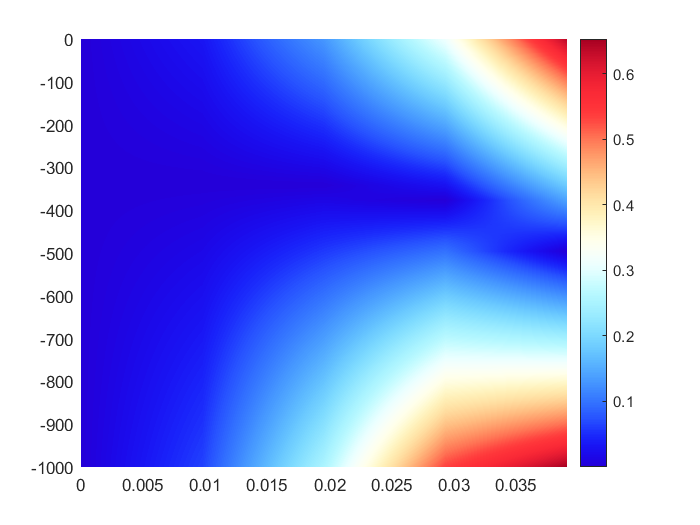
\includegraphics[width=0.6\linewidth]{Fig5_5.png}
\end{center}


\subsection{扰动的斜压纬向急流}
\subsection{Rossby波辐射的影响}
\subsection{课后习题}
\textbf{1. 以大尺度平均平行流场为例,试讨论该流场的斜压不稳定需满足的条件,
并给出不稳定扰动模态的空间尺度、传播相速度、以及空间结构。}

以两层垂直切变模型为例,两层流体中的平均纬向斜压流体:
$$u=\begin{cases}
    U \ (H/2<z<H,\ Layer \ n=1) \\
    -U \ (0 < z < H/2, \ Layer \ n=2)
\end{cases}$$

得到流函数:
$$\psi_n = (-1)^{n}Uy$$

在不受外力的作用下,其准地转位涡方程有:
$$\frac{\partial q_{QG,n}}{\partial t} + J[\psi, q_{QG,n}] = 0$$
$$q_{QG,n} 
=\nabla^2\psi_n + \beta y + (-1)^{n}\frac{f_0^2}{H_ng'}(\psi_1 - \psi_2)
=\beta y + (-1)^{n+1}\frac{Uy}{2R^2}$$

做雷诺分解,并忽略二阶扰动项有:
$$\frac{\partial q_{QG,n}'}{\partial t} 
+ J[\psi', \overline{q}_{QG,n}]
+ J[\overline{\psi}, q_{QG,n}'] = 0$$
$$$$
$$\frac{\partial q^{\prime}_{QG,n}}{\partial t_g} 
+ (-1)^{n+1}U\frac{\partial q^{\prime}_{QG,n}}{\partial x} 
+ v^{\prime}_n\left(\beta + (-1)^{n+1}\frac{U}{R^2}\right)= 0$$

假设扰动场有如下形式:
$$\psi^{\prime}_n = real(\Psi_ne^{i(kx+ly-\omega t)})$$

得到准地转位涡扰动场:
$$q_{QG,n}' = \nabla^2\psi_n' + (-1)^{n}\frac{1}{2R^2}(\psi_1' - \psi_2') 
= real((-K^2\Psi_n + (-1)^{n}\frac{1}{2R^2}(\Psi_1 - \Psi_2))e^{i(kx+ly-\omega t)})  $$

代入可以得到:
$$[CK^2 +\beta]\tilde{\Psi}_0-UK^2\tilde{\Psi}_1 = 0$$
$$[C(K^2+R^{-2}) +\beta]\tilde{\Psi}_1-U(K^2-R^{-2})\tilde{\Psi}_0 = 0$$

其中:
$$\tilde{\Psi}_0 = \frac{1}{2}(\Psi_1 +\Psi_2)$$
$$\tilde{\Psi}_1 = \frac{1}{2}(\Psi_1 -\Psi_2)$$

对于$U=0$的特殊情形,得到$\tilde{\Psi}_0\ne0$为扰动正压垂直模态振幅;$\tilde{\Psi}_1\ne0$为扰动斜压垂直模态振幅。

对于一般情形,模态振幅非平凡的情况,有:
$$[C(K^2+R^{-2}) +\beta][CK^2 +\beta]-U^2K^2(K^2-R^{-2}) = 0$$

在$\beta=0$时,解得:
$$C^2 = U^2\frac{K^2-R^{-2}}{K^2+R^{-2}}$$

在$KR<1$时,$C$为纯虚数,扰动增长或衰减;$KR>1$时,扰动震荡。

在$\beta=\ne0$时,用判别式判断$C$的虚实,有判别式$P$:
$$P=\beta^2R^{-4}+4U^2K^4(K^4-R^{-4})$$

可以得到不稳定的必要条件是$P$的最小值小于$0$,即:
$$P_{min}=\beta^2R^{-4}-U^2R^{-8}<0$$

即$U^2 > \beta^2R^4$,即斜压不稳定产生的必要条件是要有足够大的垂向剪切。

且此时波数要满足:
$$P=\beta^2R^{-4}+4U^2K^4(K^4-R^{-4})<0$$

即:
$$K^2(1-(KR)^4) > \frac{\beta^2}{U}$$

由于$beta>0$,因此仅当波动尺度大于Rossby变形半径时,才会产生斜压不稳定。
而对于波动尺度远大于Rossby变形半径和接近变形半径的尺度,需要极大的垂直剪切才能
产生斜压不稳定。在$(KR)^4 = 1/2$时最容易发生不稳定。

而对于$beta = 0$,只需要波动尺度大于Rossby变形半径,便可以产生斜压不稳定。

斜压不稳定的传播相速度为:
$$C = \frac{\beta(2K^2+R^{-2})}{2K^2(K^2+R^{-2})}\pm\frac{i\sqrt{-P}}{2K^2(K^2+R^{-2})}$$

其空间结构为上层扰动相对于下层扰动向西偏移0到1/2个波长。

\newpage

\section{边界层与风生环流动力学}
\subsection{行星边界层}
\subsubsection{边界层近似}
\subsubsection{切变边界层}
\subsubsection{涡粘度封闭性}
对于平均方程,由于雷诺应力未知,平均流方程并不封闭,从而引发湍流封闭性问题(Turbulence closure problem)。

涡粘度封闭性假定:认为雷诺应力像分子粘性力那样输送动量,具体地,假定涡动动量通量和平均流切变之间存在下面的关系:
$$\overline{{w}^{\prime}{u}^{\prime}}=-{{\nu }_{e}}\frac{\partial \overline{u}}{\partial z}$$

其中,${\nu }_{e}$是涡粘度,当$Re \gg 1$时,涡粘度大于分子粘性系数。从而得到没有显式湍流分量解的平均流边界层问题,这类边界层问题成为参数化的行星边界层。在响应的涡动$Re$数低于边界层速度不稳定性的阈值是,该参数化方案是合理的。随着$Re$数的增加,层流变为过渡期的不稳定,$Re$数继续增大发展成湍流。

\subsubsection{底边界Ekman层}
根据涡粘度封闭性,我们有Ekman层方程组:
\begin{align}
  & f\overline{v}=\text{-}{{\nu }_{e}}\frac{{{\partial }^{2}}\overline{u}}{\partial {{z}^{2}}}, \\ 
 & f\overline{u}={{\nu }_{e}}\frac{{{\partial }^{2}}\overline{v}}{\partial {{z}^{2}}}, \\ 
 & \overline{w}=-\int_{0}^{z}{(\frac{\partial \overline{u}}{\partial x}+\frac{\partial \overline{v}}{\partial y})}d{z}^{\prime}, \\ 
 & {{\overline{u}}_{h}}=-\overline{u}_{h}^{i},\ \ \ z=0, \\ 
 & {{\overline{u}}_{h}}\to 0,\ \ \ \ z\to \infty .\ \ \ \  
\end{align}

可以得到Ekman螺线解,在北半球,自边界层底部向上,边界层异常速度随高度增加而减小并顺时针旋转;在南半球相反。

以及底边界层应力:
$$\tau_s=\rho_0\nu_e\frac{\partial\bar{u}}{\partial z}=\rho_0\sqrt{\frac{f\nu_e}{2}}\begin{bmatrix}
    1&-f/|f|\\
    f/|f|& 1
\end{bmatrix}u_g$$

在北半球,$\tau_s$相对于地转流逆时针旋转了$45^{\circ}$;在南半球$\tau_s$相对于地转流顺时针旋转了$45^{\circ}$。

底边界层输运:
$$T=\frac{1}{\rho_0f}\begin{bmatrix}
    0&-1\\
    1& 0
\end{bmatrix}\tau_s$$

在北半球,$T$相对于$\tau_s$逆时针旋转了$90^{\circ}$;在南半球,$T$相对于$\tau_s$顺时针旋转了$90^{\circ}$

Ekman抽吸:
\begin{align}
  & {{\overline{w}}^{b}}(\infty )=\widehat{z}\cdot \nabla \times \left[ \frac{{{\tau }_{s}}}{{{\rho }_{0}}f} \right] \\ 
 & \ \ \ \ \ \ \ \ \ \ =\frac{\partial }{\partial x}\left[\frac{{{\varepsilon }_{ek,bot}}}{f}({{S}_{f}}{{\overline{u}}^{i}}+{{\overline{v}}^{i}})\right]-\frac{\partial }{\partial y}\left[\frac{{{\varepsilon }_{ek,bot}}}{f}({{\overline{u}}^{i}}-{{S}_{f}}{{\overline{v}}^{i}})\right] \\ 
 & \ \ \ \ \ \ \ \ \ \ =\frac{{{\varepsilon }_{ek,bot}}}{f}({{S}_{f}}\frac{\partial {{\overline{u}}^{i}}}{\partial x}+\frac{\partial {{\overline{v}}^{i}}}{\partial x}-\frac{\partial {{\overline{u}}^{i}}}{\partial y}+{{S}_{f}}\frac{\partial {{\overline{v}}^{i}}}{\partial y})+\frac{\beta {{\varepsilon }_{ek,bot}}}{{{f}^{2}}}({{\overline{u}}^{i}}-{{S}_{f}}{{\overline{v}}^{i}}) \\ 
 & \ \ \ \ \ \ \ \ \ \ =\frac{{{\varepsilon }_{ek,bot}}}{f}{{\overline{\zeta }}^{i}}+\frac{\beta {{\varepsilon }_{ek,bot}}}{{{f}^{2}}}({{\overline{u}}^{i}}-{{S}_{f}}{{\overline{v}}^{i}}).\ \ \ \  
\end{align}

其中${\varepsilon }_{ek,bot}=\sqrt{\frac{|f|\nu_e}{2}}$

\subsubsection{海表Ekman层}
之前的分析是针对固体边界上方的流体的,适用于大气和海洋的底部。甚至对于液体海洋上方的风来说,海洋表层洋流通常比海洋上方的风要慢得多。因而无滑移边界条件是对大气动力的一 个好的近似,因此之前的分析也适用于海洋上方的大气边界层。

对于液体顶部的边界,特别是由海表风应力驱动的海洋顶部,可以进行类似的分析。海洋上方的大气边界层所产生的海表风应力驱动了海洋行星边界层。

海表Ekman基本方程为:
\begin{align}
  & f\overline{v}=\text{-}{{\nu }_{e}}\frac{{{\partial }^{2}}\overline{u}}{\partial {{z}^{2}}}, \\ 
 & f\overline{u}={{\nu }_{e}}\frac{{{\partial }^{2}}\overline{v}}{\partial {{z}^{2}}}, \\ 
 & \rho_0\nu_e\frac{\partial u}{\partial z} = \tau_s\ \ \ z=0, \\ 
 & {{\overline{u}}_{h}}\to 0,\ \ \ \ z\to -\infty .\ \ \ \  
\end{align}

可以得到Ekman螺线解,对海表Ekman层来说:海洋中的Ekman螺线始于一个与海表风应力向右
(左)旋转了$45$度的表面速度,随着深度的增加,速度减小并且顺(逆)时针旋转,直至在海洋深
层速度减小为$0$。

海表的Ekman速度:
$$\overline{u}(0)=\frac{1}{{{\rho }_{0}}\sqrt{2\left| f \right|{{\nu }_{e}}}}\left( \begin{matrix}
   1 & {{S}_{f}}  \\
   -{{S}_{f}} & 1  \\
\end{matrix} \right){{\tau }_{s}}$$

以及海表的Ekman输运:
$$T=\frac{1}{\rho_0f}\begin{bmatrix}
    0& 1\\
    -1& 0
\end{bmatrix}\tau_s$$

在北半球,$T$相对于$\tau_s$顺时针旋转了$90^{\circ}$;在南半球,$T$相对于$\tau_s$逆时针旋转了$90^{\circ}$

海表的Ekman抽吸:
$${{\overline{w}}^{b}}(-\infty )={{w}_{ek,top}}=\hat{k}\cdot \nabla \times \left[ \frac{{{\tau }_{s}}}{{{\rho }_{0}}f} \right]$$

由于海表Ekman层问题和总表面速度无关(因为忽略了洋流对确定表面应力的贡献),因此其Ekman洋流可以强加于任一内部地转洋流之上。

另一种说法是,驱动海洋行星边界层湍流的切变不稳定性通常是由于平均边界层切变而不是内部地转切变产生的,即使后者在一个分层的海洋中是斜压的,因此其Ekman洋流可以强加于任一内部地转洋流之上。

\subsubsection{涡旋转减弱(Spin down)}
大气底部的Ekman层,通过Ekman抽吸向气旋中心输送质量,使得大气内部流体环流强度减弱。
\begin{center}
    \includegraphics[width=10cm]{Fig5_2.png}
\end{center}
旋转减弱(Spin down): Ekman pumping导致边界层顶的垂直运动,使得内部自由流体的旋转强度减弱。

考虑一个正压涡度方程:
$$\frac{d(\zeta +f)}{dt}=-(f+\zeta ){{\nabla }_{h}}\cdot\mathbf{u}$$

在$f$平面近似下,有:
$$\frac{\partial(\zeta +f)}{\partial t}\approx-f{{\nabla }_{h}}\cdot\mathbf{u}=f\frac{\partial w}{\partial z}\approx-\frac{f}{H-h}w_{ek}=-\frac{{\varepsilon }_{ek,bot}}{H-h}\zeta$$

其中$H$为抽吸为$0$的高度,$h$为抽吸开始的高度。

1)涡旋形状不变,强度随时间呈指数衰减;

2)旋转衰减时间$t_d$:涡旋强度衰减至初始强度的$1/e$所需的时间;

3)$t_d$只取决于$f$ 和 $h_{ek}$,远大于旋转周期$1/f$

对于非常强的涡旋(如飓风),也可以进行类似上述的分析。分析结果表明,涡旋形状改变。涡旋强度也随时间减弱,但并非为指数形式衰减,且衰减时间依赖于涡旋自身的强度。

\subsubsection{湍流Ekman层}

\subsection{海洋风生环流和西边界层}
\subsubsection{环流问题的提出}
假设在一个矩形区域同时取刚盖近似,海水有均一的密度,海表存在定常的风应力

1. 研究北半球的情形,$f>0$

2. 取$\beta$平面近似

3. 在底边界$z=0$处速度$u=0$

4. 在海表面$z=H$处存在风应力$\tau$

将整个海洋分为三层,即海表边界层,海底边界层和内层,内层位于两个边界层中间,并且边界层的厚度远小于内层的厚度。
\begin{center}
    \includegraphics[width=8cm]{Fig5_1.png}
\end{center}

根据Taylor-Proudman定理可以知道,在内层中,水平速度和水平压力梯度与深度无关(即正压)。根据流体的连续性,在内层中,垂直速度随深度呈线性变化。在边界层,由于Reynolds应力较大,使得方程中的动量平衡存在非地转分量,因此Ekman层中的运动不满足Taylor-Proudman定理。

考虑存在一个如下形式的风应力:
$$\tau_s = \tau_s^x(y) \hat{i}$$
\begin{center}
    \includegraphics[width=0.5\linewidth]{Fig5_3.png}
\end{center}

海表Ekman层和海底Ekman层的水平输送可表示为:
\begin{align}
  & {{\mathbf{T}}_{ek,top}}=-\mathbf{\hat{z}}\times \frac{{{\mathbf{\tau }}_{s}}}{{{\rho }_{0}}f} \\ 
 & {{\mathbf{T}}_{ek,bot}}=\frac{{{\varepsilon }_{ek,bot}}}{f}(-u_{bot}^{i}-v_{bot}^{i},u_{bot}^{i}-v_{bot}^{i})\ \  
\end{align}

Ekman抽吸的速度为:
\begin{align}
  & {{w}_{ek,top}}=\mathbf{\hat{z}}\cdot \nabla \times \left[ \frac{\tau _{s}^{x}\mathbf{\hat{x}}}{{{\rho }_{0}}f} \right]=-\frac{1}{{{\rho }_{0}}}\frac{\partial }{\partial y}\left[ \frac{\tau _{s}^{x}}{f} \right] \\ 
 & {{w}_{ek,bot}}=\frac{{{\varepsilon }_{ek,bot}}}{f}\zeta _{bot}^{i}+\frac{\beta {{\varepsilon }_{ek,bot}}}{{{f}^{2}}}\left( u_{bot}^{i}-v_{bot}^{i} \right)\ \  
\end{align}

内层中的位涡方程可以写为:
$$\frac{\partial {{\zeta }^{i}}}{\partial t}+\mathbf{u}_{h}^{i}\cdot \nabla \left( f(y)+{{\zeta }^{i}} \right)=-\left( f+{{\zeta }^{i}} \right)\nabla \cdot \mathbf{u}_{h}^{i}+{{\mathcal{F}}^{i}}$$

进一步假设流体是定常的,内层中的非保守力项可以忽略,流体的运动较弱,非线性项的作用也可以忽略。那么:
$$\beta H{{v}^{i}}=-\frac{1}{{{\rho }_{0}}}\frac{\partial \tau _{s}^{x}}{\partial y}+\frac{\beta \tau _{s}^{x}}{f{{\rho }_{0}}}-{{\varepsilon }_{ek,bot}}{{\zeta }^{i}}-\frac{\beta {{\varepsilon }_{ek,bot}}}{f}({{u}^{i}}-{{v}^{i}})$$

而整层海洋的经向输送可以表达为:
$$HV=H{{v}^{i}}+T_{ek,top}^{y}+T_{ek,bot}^{y}$$

代入上述方程得到:
$$\beta HV=-\frac{1}{{{\rho }_{0}}}\frac{\partial \tau _{s}^{x}}{\partial y}-{{\varepsilon }_{ek,bot}}{{\zeta }^{i}}$$

最后,假设流体的上下边界都是平坦的,根据运动边界条件,对连续方程进行垂直积分,可以得到深度平均的水平速度$U$,$V$是水平无辐散的。
$${{T}^{x}}=HU=-\frac{\partial \Psi }{\partial y},\ {{T}^{y}}=HV=\frac{\partial \Psi }{\partial x}$$

这里的$\Psi = H\psi$,为输送流函数(满足正压条件)。

底部Ekman层的速度与内层中的速度具有相同的量级(以满足底部的无滑动边界条件),而底边界的输送相对于内层的输送为$h_{ek,bot}/H=\sqrt{E}<<1$,可以忽略。但由于海表Ekman层的速度相对于内层大很多,因此海表的Ekman层输送相对于内层的输送是不可忽略的。

忽略底边的Ekman输送,得到:
$${{\nabla }^{2}}\Psi \approx H{{\zeta }^{i}}+\mathbf{\hat{z}}\cdot \nabla \times \frac{\tau _{s}^{x}\mathbf{\hat{x}}}{{{\rho }_{0}}f}$$

代入:
$$\beta HV=-\frac{1}{{{\rho }_{0}}}\frac{\partial \tau _{s}^{x}}{\partial y}-{{\varepsilon }_{ek,bot}}{{\zeta }^{i}}$$

得到:
$$\frac{{{\varepsilon }_{ek,bot}}}{H}{{\nabla }^{2}}\Psi +\beta \frac{\partial \Psi }{\partial x}=-\frac{1}{{{\rho }_{0}}}\frac{\partial \tau _{s}^{x}}{\partial y}+\frac{{{\varepsilon }_{ek,bot}}}{H}\mathbf{\hat{z}}\cdot \nabla \times \frac{\tau _{s}^{x}\mathbf{\hat{x}}}{{{\rho }_{0}}f}$$

\subsubsection{内区和边界层环流}
对于一个具有平坦底边界和理想风应力的矩形海域,其定常的线性正压解为:
$$\frac{{{\varepsilon }_{ek,bot}}}{H}{{\nabla }^{2}}\Psi +\beta \frac{\partial \Psi }{\partial x}=-\frac{1}{{{\rho }_{0}}}\frac{\partial \tau _{s}^{x}}{\partial y}$$

在气候平均上,中纬度为西风带,热带和极地为东风带,可假设风应力具有以下的表达式($y=0$对应着中纬度西风最强的地区):
\begin{align}
  & \ \ \ \ \tau _{s}^{x}(y)={{\tau }_{0}}\cos \left[ \frac{2\pi y}{{{L}_{y}}} \right] \\ 
 & \Rightarrow \frac{\partial \tau _{s}^{x}}{\partial y}\text{=}-\frac{2\pi {{\tau }_{0}}}{{{L}_{y}}}\sin\left[ \frac{2\pi y}{{{L}_{y}}} \right]\ \  
\end{align}

这样的风应力可以强迫出海洋上的双环流结构,即在北部为一个气旋式环流,南部为一个反气旋式环流。

1. Sverdrup输送:

将输送流函数改成一般的形式有:
$$D{{\nabla }^{2}}\psi +\frac{\partial \psi }{\partial x}=A\sin \left[ \frac{2\pi y}{{{L}_{y}}}\right] $$

这样一个椭圆偏微分方程,是可以得到它的解析解,但十分复杂。然而,对于这样一个问题,同时通过尺度分析 $D \ll L_x$并且$E \ll 1$,从而可以采用边界层近似的方法,得到方程的近似解,这个近似解可以帮助我们更好地理解海洋环流的特点。

考虑O(D),方程简化为:
$$\frac{\partial \psi }{\partial x}=A\sin \left[ \frac{2\pi y}{{{L}_{y}}} \right]$$

这种近似对于内区流体是成立的,但对于侧边界是不一定成立的。对该方程在$x$方向上进行积分,
$$\psi ={{\psi }^{i}}\left( x,y \right)=-A({{L}_{x}}-x)\sin \left[ \frac{2\pi y}{{{L}_{y}}} \right]$$

这种水平环流称作Sverdrup输送。

两边同乘以$H$,得到环流的体积输送:
$$\Psi \left( x,y \right)=-\frac{1}{{{\rho }_{0}}\beta }\int_{x}^{{{L}_{x}}}{dx\left[ \mathbf{\hat{z}}\cdot {{\nabla }_{h}}\times {{\mathbf{\tau }}_{s}} \right]}$$

在海洋内区,正压流函数是风应力旋度的线性函数。

2. Munk理论

为了得到完整解的情况,在$x=0$处取边界层近似。定义一个无量纲坐标$\xi=x/D$。

假设解存在以下的形式:$\psi = \psi^i +\psi^b$

代入一般的流函数方程得到:
$${{D}^{-1}}\left[ \frac{{{\partial }^{2}}{{\psi }^{b}}}{\partial {{\xi }^{2}}}+\frac{\partial {{\psi }^{b}}}{\partial \xi } \right]+{{D}^{0}}\left[ \frac{\partial {{\psi }^{i}}}{\partial x}-A\sin \left[ \frac{2\pi y}{{{L}_{y}}} \right] \right]+{{D}^{1}}\left[ {{\nabla }^{2}}{{\psi }^{i}}+\frac{{{\partial }^{2}}{{\psi }^{b}}}{\partial {{y}^{2}}} \right]=0$$

在边界处,由于O(D),$D^1$项可以忽略,从而只剩下:
\begin{align}
  & \frac{{{\partial }^{2}}{{\psi }^{b}}}{\partial {{\xi }^{2}}}+\frac{\partial {{\psi }^{b}}}{\partial \xi }=0 \\ 
 & \ \ \ \ \ \ \ {{\psi }^{b}}=-{{\psi }^{i}}(0)\ \ at\ \ \xi =0 \\ 
 & \ \ \ \ \ \ \ {{\psi }^{b}}\to 0\ \ as\ \ \xi \to \infty \ \ \ \  
\end{align}

最后得到近似解:
$$\psi \left( x,y \right)=-A{{L}_{x}}\sin \left[ \frac{2\pi y}{{{L}_{y}}} \right]\left( 1-\frac{x}{{{L}_{x}}}-{{e}^{{-x}/{D}\;}} \right)$$

$\psi$的空间分布如下图所示,它是由两个环流圈所组成的,北部的副极地环流圈是气旋式的,南部的副热带环流圈是反气旋式的。

在$y=0$处,是西风的极大值位置,对应着风场涡度为零的地区,也就是南北环流的分界线。每一个环流都有一个较窄的西边界流,这里的流线和西边界平行。
\begin{center}
    \includegraphics[width=0.5\linewidth]{Fig5_4.png}
\end{center}

3. 为什么强边界流出现在西边界?

考虑一般形式的流函数:
$$D{{\nabla }^{2}}\psi +\frac{\partial \psi }{\partial x}=A\sin [ \frac{2\pi y}{{{L}_{y}}}] $$

在$x$方向上积分,左侧的第二项为$0$。在北半球,参数$D$和$A$均大于$0$,故${\nabla }^{2}\psi$和$A\sin [ \frac{2\pi y}{{{L}_{y}}}]$同号,故在副热带$\psi$为顺时针环流,在副极地地区为逆时针环流。

而对于简化的方程:
$$\frac{\partial \psi }{\partial x}=A\sin \left[ \frac{2\pi y}{{{L}_{y}}} \right]$$

从东边界积分,对应于北逆南顺的双环流;从西边界积分,对应于北顺南逆的双环流。所以,从东边界积分合理,强边界流出现在西边界。

\subsubsection{在实际环流中的应用}
\subsubsection{湍流斜压风生环流}

\subsection{课后习题}
\textbf{1. 讨论海表Ekman抽吸如何影响海洋内层气旋的变化,并给出原因。}

海表为刚盖,无限深处考虑Ekman抽吸:
$$w(-\infty) = \int_{-\infty}^0(\frac{\partial u}{\partial x} 
+ \frac{\partial v}{\partial y})dz$$

有Ekman基本关系:
\begin{align}
    & f\overline{v}=\text{-}{{\nu }_{e}}\frac{{{\partial }^{2}}\overline{u}}{\partial {{z}^{2}}}, \\ 
   & f\overline{u}={{\nu }_{e}}\frac{{{\partial }^{2}}\overline{v}}{\partial {{z}^{2}}}, \\ 
   & \rho_0\nu_e\frac{\partial u}{\partial z} = \tau_s\ \ \ z=0, \\ 
   & {{\overline{u}}_{h}}\to 0,\ \ \ \ z\to -\infty .\ \ \ \  
\end{align}

可以解得Ekman抽吸:
$$w(-\infty)={{w}_{ek,top}}=\hat{k}\cdot \nabla \times \left[ \frac{{{\tau }_{s}}}{{{\rho }_{0}}f} \right]$$

考虑海洋内层存在一个涡旋,远离海表,满足正压涡度方程,风应力对其无外力作用:
$$\frac{\partial(\zeta+f)}{\partial t} + \nabla_h\cdot((f+\zeta)\vec{u})
 = \frac{\partial(\zeta+f)}{\partial t} + \nabla_h\cdot\zeta\vec{u}
 + \nabla_h\cdot f\vec{u}=0$$

得到:
$$\frac{\partial\zeta}{\partial t} + \nabla_h(\zeta\vec{u})
=-\beta v +f\frac{\partial w}{\partial z}$$

在涡旋区域内积分,假设涡旋在Ekman层以下,Ekman抽吸作用在涡旋表层,得到:
$$\frac{d}{dt}\iiint\zeta dxdydz
=-\beta\iiint v dxdydz + f\iint w(-\infty) dxdy$$

假设风应力远大于地转效应,得到涡度变化:
$$\frac{d}{dt}\iiint\zeta dxdydz
= f\iint  w(-\infty) dxdy$$

得到,在北半球,在海表Ekman抽吸为正时,涡度增大,涡度气旋性加强,反气旋减弱;
海表Ekman抽吸为负时,涡度降低,涡度气旋性减弱,反气旋增强。
在南半球,在海表Ekman抽吸为正时,涡度减小,涡度气旋性加强,反气旋减弱;
海表Ekman抽吸为负时,涡度减弱,涡度气旋性减弱,反气旋增强。

将Ekman抽吸写成气旋的形式:
$$\frac{d}{dt}\iiint\zeta dxdydz
=\iint\hat{k}\cdot \nabla \times \left[ \frac{{{\tau }_{s}}}{{{\rho }_{0}}} \right]dxdy$$

可以得到,当海表风应力旋度和气旋方向一致时,气旋性加强,反气旋减弱;
当海表风应力旋度和气旋方向相反时,气旋性减弱,反气旋增强。

\textbf{2. 假定观测$w^{obs}$,该观测的演变由一个线性方程所描述,
即$\frac{dw^{obs}}{dt} = Aw^{obs} + F$,其中矩阵$A$是$n\times n$实数矩阵,
外强迫F是n维物理向量,设计该观测的预报模式,给出预报误差发展的控制方程,
并分析预报误差的来源}

对于预报$t_{n+1}$时刻的观测,将预报方程写成差分格式,有:
$$\frac{w_{n+1} - w_{n}}{\Delta t} = Aw_{n} + F_n$$
$$w_{n+1} = (I_n+\Delta tA)w_{n} + \Delta tF_n$$

即根据$t_0$时刻的观测,可以推演到$t_{n+1}$时刻的观测。

将该方程和观测演变方程相减,得到预报误差的发展方程:
$$\frac{d\delta w}{dt} = A\delta w$$

预报的误差来自多个方面,初始误差,强迫场误差,模式误差。

\end{document}